% This is a "bare-bones" thesis template file.  For examples of how to
% use a few more LaTeX features, look in the 'sample' folder.  Read
% the User Guide for documentation of the 'fsuthesis' class features.

\documentclass[11pt,expanded,copyright]{fsuthesis}

% Additional packages may be loaded here.
\usepackage{graphicx}
\usepackage{cite}
\usepackage{longtable}
\usepackage{amsmath}
\usepackage{multirow}
\usepackage{multicol}
%\usepackage{wrapfig}
\usepackage{float}
\usepackage{algorithmicx}
\usepackage{algpseudocode}
%\usepackage[section]{placeins}
%\usepackage{subcaption}
\usepackage{array}
\usepackage[export]{adjustbox}
\usepackage{tabu}
\usepackage{tabularx}
\usepackage{listings}
\usepackage{siunitx}
\usepackage{siunitx}
\usepackage{ wasysym }
\usepackage[section]{placeins}
\usepackage[usenames, dvipsnames]{color}




% Do NOT use 'geometry' or 'setspace' packages! They will
% mess up the spacing provided by 'fsuthesis'.

\title{MANAGEMENT OF DISTRIBUTED ENERGY RESOURCES}
\author{Alvi Newaz}
\college{College of Engineering}
\department{Department of Electrical and Computer Engineering} % Delete if no department
\manuscripttype{Prospectus examination report}              % [Thesis, Dissertation, Treatise]
\degree{Doctor of Philosophy}                 
\degreeyear{2019}
\defensedate{March 31, 2015}

%\subject{My Topic}
%\keywords{keyterm1; keyterm2; keyterm3; ...}

\committeeperson{Omar Faruque}{Professor Directing Thesis}
\committeeperson{Juan C. Ordonez}{University Representative}
\committeeperson{Sastry Pamidi}{Committee Member}
\committeeperson{Simon Y. Foo}{Committee Member}

\clubpenalty=9999
\widowpenalty=9999

\begin{document}

\frontmatter
\maketitle
\makecommitteepage

%\begin{dedication}
%\end{dedication}

%\begin{acknowledgments}
%\end{acknowledgments}

\tableofcontents
\listoftables
\listoffigures
%\listofmusex

%\begin{listofsymbols}
%\end{listofsymbols}

%\begin{listofabbrevs}
%\end{listofabbrevs}

\begin{abstract}
Distributed energy resources (DERs) is one of the fastest growing components in distribution systems. The growth of DER integration has also brought with it some new concerns. With the introduction of fast-changing DERs and reverse power flow voltage regulation is facing some issues. Also how to optimally use the available DERs with the presence of a real-time pricing scheme is also a topic of interest. This report presents the challenges associated with the two topics mentioned and provides novel solutions to tackle the issues.

With the integration of DERs into the grid, the traditional notion of unidirectional power flow is no longer valid. The concept that power is generated in one central location and then provided to the consumers through transmission and distribution networks is no longer valid. DERs make it possible to generate and store power near the source. Solar and wind are two of the most prominent DERs available in the distribution grid. However, they are non-dispatchable and fast changing. This causes the traditional regulation devices to operate more than necessary. Moreover, the slow response time of traditional voltage regulation schemes is not suitable to cope with the fast-changing DERs. To combat this issue, this report presents a novel voltage regulation technique based on the concepts of electrical distance calculation and voltage sensitivity analysis.

Another DER that is becoming prominent in the grid is distributed storage (DS). DS can be used to combat the non-dispatchable fast-changing nature of solar and wind energy resources. It also has the potential to reduce the cost for both the consumer and utility by storing power when it is cheap and supplying when power is costly. However, the optimization of DS with the other DERs present in the grid is still a contemporary research topic. This report presents a graph search based energy management method which takes into account the present status and future forecasts to optimally use available DERs.

This research report presents the current status of development of the voltage regulation algorithm and the graph search based energy management scheme. It also presents preliminary validation results.
\end{abstract}

\mainmatter

\chapter{Introduction}
\label{TH_intro}
\section{Integration of Distributed Energy Resources in Distribution System}
With the growing population, and increasing modernization and industrialization, the global power demand is estimated to increase drastically, more than triple by the ends of this century \cite{INTRO1}. The present power industry is faced with the great challenge of balancing power generation with this increasing demand. In 2017 an estimated 4 trillion kilowatt hours of electricity was generated to meet the demands of the United States \cite{EIA2018}. Table \ref{tab:IN1} shows the percentage of the different sources of generation in the US for the year 2017. The data used in the table is collected from \cite{EIA2018}.

\begin{table}[ht]
\label{tab:IN1}
\caption[U.S. electricity generation by source, amount, and share of total in 2017]{U.S. electricity generation by source, amount, and share of total in 2017 \cite{EIA2018}}
\centering
\begin{tabular}{|c|c|c|}
\hline
Energy source & Billion kWh & Share of total \\ \hline
Total - all sources & 4,034 &  \\ \hline
Fossil fuels (total) & 2,536 & 62.90\% \\ \hline
Natural gas & 1,296 & 32.10\% \\ \hline
Coal & 1,206 & 29.90\% \\ \hline
Petroleum (total) & 21 & 0.5\% \\ \hline
Petroleum liquids & 12 & 0.3\% \\ \hline
Petroleum coke & 9 & 0.2\% \\ \hline
Other gases & 12 & 0.3\% \\ \hline
Nuclear & 805 & 20.0\% \\ \hline
Renewables (total) & 687 & 17.0\% \\ \hline
Hydropower & 300 & 7.4\% \\ \hline
Wind & 254 & 6.3\% \\ \hline
Biomass (total) & 63 & 1.6\% \\ \hline
Wood & 41 & 1.0\% \\ \hline
Landfill gas & 12 & 0.3\% \\ \hline
Municipal solid waste (biogenic) & 7 & 0.2\% \\ \hline
Other biomass waste & 3 & 0.1\% \\ \hline
Solar (total) & 53 & 1.3\% \\ \hline
Photovoltaic & 50 & 1.2\% \\ \hline
Solar thermal & 3 & 0.1\% \\ \hline
Geothermal & 16 & 0.4\% \\ \hline
Pumped storage hydropower & -6 & -0.2\% \\ \hline
Other sources & 13 & 0.3\% \\ \hline
\end{tabular}
\end{table}

From the table \ref{tab:IN1}, it is evident that the current energy sources mostly rely on natural gas and coal. These are resources that do not renew at a sufficient rate to allow sustainable extraction. The increased power demand combined with the non-renewable nature of the energy resources and their adverse effect on the environment necessitates the incorporation of new and alternative resources to meet the future demand. This has been a significant drive for renewable distributed energy resource (DER) integration into the grid \cite{khan2009review,bignucolo2008radial,series2009microgrids}. With the growth in power demand, the penetration of distributed energy resource in the distribution system is rising. This trend of adding energy resources in the distribution system is changing the current infrastructure of modern power systems. Fig. \ref{fig:NEW_GRID} shows this transformation of the power grid and what it might look like in the near future. 

\begin{figure}[!h]
\centering
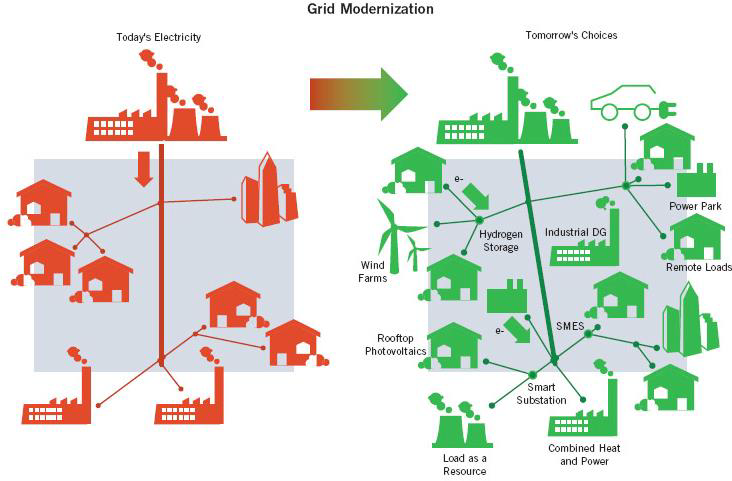
\includegraphics[width=0.85\linewidth]{figs/NEW_GRID.png}
\caption[Power grid modernization.]{Power grid modernization.\cite{NEW_GRID}}
\label{fig:NEW_GRID}
\end{figure}

With the integration of DERs power is no longer only generated in bulk at generation facility and then through transmission and distribution supplied to the consumer. DERs make it possible to generate power near the demand. This increases system stability and reduces system loss as power does not need to travel far to reach the source. DERs can be divided into distributed generation (DG) and distributed energy storage (DES). 

\subsection{Distributed Generation}
Distributed generation is an approach that employs appropriate small and medium scale electricity generation resources near the consumer. Non-renewable fuel based distributed generation technologies and dispatchable renewable distributed generation has been a part of the grid for many years. In recent years the incorporation of variable renewable energy based DG has increased significantly. There are mainly two types of variable renewable DGs used in the distribution grid.
\begin{enumerate}
    \item Solar Energy Based DGs
    \item Wind Energy Based DGs
\end{enumerate}
Besides these, biomass, small scale hydro and combined heat and power are some of the prominent distributed generation plants being added to the grid. Fig. \ref{fig:GROWTH_EIA} shows the current trend as well as the projected future of electricity generation by source. It is evident from the figure that renewable generation sources will keep on increasing in the grid. 

\begin{figure}[!h]
\centering
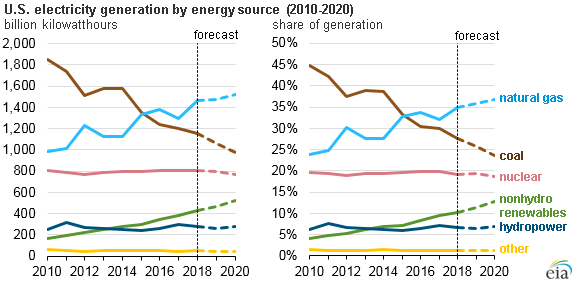
\includegraphics[width=0.85\linewidth]{figs/GROWTH_EIA.png}
\caption[Us electricity generation by energy source.]{Us electricity generation by energy source.\cite{EIA2018}}
\label{fig:GROWTH_EIA}
\end{figure}

\subsection{Distributed Energy Storage}
Energy storage can provide backup power and increase grid stability by mitigating the effects of variable renewable generation in the grid. It can also be used to store energy during relatively low demand and release it back during high demand periods. There are various energy storing methods currently used in the grid, including \cite{GE1}:
\begin{itemize}
    \item \textbf{Pumped Hydro:} In times of low demand and high generation electricity is used to pump water in a storage reservoir. During high demand, the stored water is used to generate power.
    \item \textbf{Compressed Air:} During low demand electricity is used to store compressed air up to 1,000 Psi. Then it is used to generate during low demand.
    \item \textbf{Batteries:} Batteries store electricity in the form of chemical energy. Similar to the previous approaches, electricity is stored during low demand and released during high demand.
    \item \textbf{Flywheels:} Flywheel uses electricity to store rotational kinetic energy. During low demand, a motor is used to rotate the flywheel and store kinetic energy. During high demand, this kinetic energy is used to rotate a generator and produce power.
    \item \textbf{Thermal Storage:} During times of low demand, electricity is used to store thermal energy. Then during high demand, the stored energy is used for heating and cooling applications.
\end{itemize}

As of June 2016, the US had over 21.6 GW of rated power in energy storage. Most of the projects are Electro-chemical energy storage projects. Pumped hydro storage represents the majority capacity of the currently available storage. Fig. \ref{fig:ES_INCREASE} shows the growth of energy storage installation in the grid. Between the years 2008 – 2016, the US has installed 1.17 GW new energy storage capacity in the grid. 

\begin{figure}[!h]
\centering
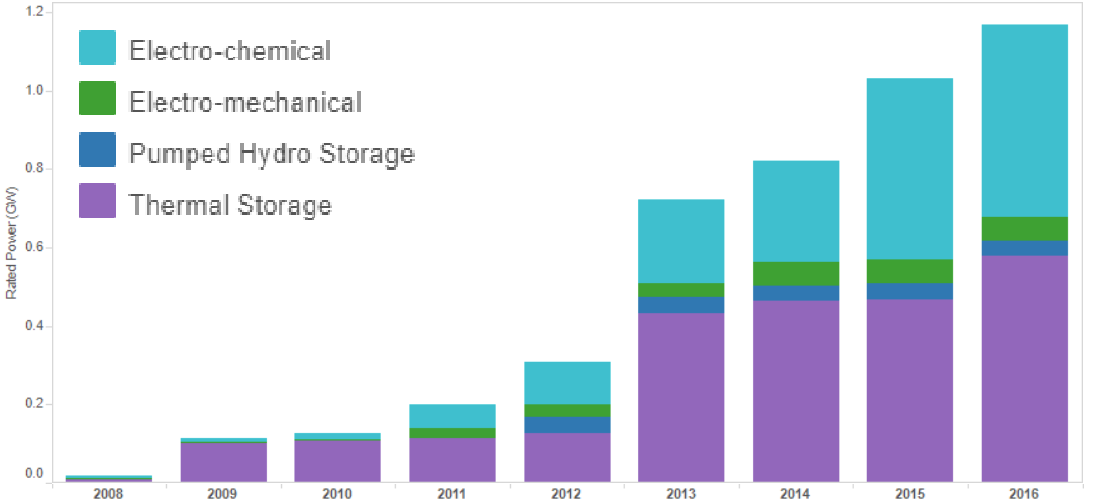
\includegraphics[width=0.85\linewidth]{figs/ES_INCREASE.png}
\caption[Recently installed grid energy storage in the U.S.]{Recently installed grid energy storage in the U.S \cite{GE2}}
\label{fig:ES_INCREASE}
\end{figure}


\section{Issues Due to High Penetration of DERs in Distribution system}
The current power grid was designed to accommodate unidirectional power flow. This was an efficient design to distribute power from central transmission to distribution feeders to the loads \cite{HPPV}.  With the introduction of DGs, the traditional design has to face some new challenges. The existing distribution system components were not designed to accommodate bidirectional power flow \cite{HPPV}. Therefore, concerns are arising regarding the increased penetration of DGs. This is a vital research field. This field is getting more attention as more DGs are incorporated into the grid. 

The potential impact of the integration of DGs in the distribution system is affected by many different parameters. The location and rating of the DG, the regulation and protection equipment present in the system, the stiffness of the feeder, etc. play a significant role in the impact of the DG. Moreover, the variability of the non-dispatchable variable DGs also plays a significant role in the negative impact the DGs might have on the feeder. This chapter will present a review of the potential impacts of DG integration, mostly focusing on voltage regulation issues.

\subsection{General Potential Impacts}
There are a lot of potential impacts that may happen in a distribution grid with a high penetration of DGs. This brief review presents a small part of the impacts. In this section, some of the general system-level impacts are stated with references that deeply explain the phenomenon. Some of the impacts may be:
\begin{itemize}
    \item Voltage ride through: Voltage ride through or low voltage ride through is the capability of electric generators to stay connected to the grid during short periods of under voltage or voltage dip. This feature is specially necessary in systems with high penetration of fast changing renewable generations. This would require the use of proper grounding and smart inverters with voltage ride through capabilities \cite{GPI1}.   
    \item Tripping of multiple DGs: The conventional power system had been designed considering stable power flow. But with higher penetration of DGs large random fluctuation of real power can occur in the system. This can lead to tripping of multiple DGs in the system and cause power-loss \cite{GP2}.
    \item Protection system coordination: The traditional protection devices available in the distribution network are circuit breakers, reclosers, sectionalizes and fuses. The traditional grid protection is coordinated using inverse definite minimum time (IDMT) curves. These curves are used to rate the protection devices to protect against over current and earth faults. The IDMT based solutions were optimized to make sure minimum number of customers were affected by the faults. The traditional network had only one source of fault current. So the IDMT based solutions did not take into account the effects of DERs. These protection schemes have been shown to be insufficient with a high DG penetration in \cite{PR133} and \cite{PR134}.
    \item DC injection: Inverter interfaced DGs can inject DC currents in the system \cite{GP5}. Even a small DC voltage can inject a large DC current as the network impedance of an AC network is low. This can cause saturation in devices such as transformers and motors.
    \item Line overloading: If excess generation from DGs are injected into the grid it can cause the lines to overload. \cite{GP6}
\end{itemize}
The effects of DG integration can appear at any level of penetration but as the DG generation start to overcome the demand of the nearby loads the effects start to become more prominent \cite{Th_ali}.

\subsection{Technical potential impact}
Besides these, there are some technical potential impacts that need to be considered.

\subsubsection{Impacts on Power Quality}
“Power quality is a set of electrical boundaries that allow a piece of equipment to function in its intended manner without significant loss of performance or life expectancy” \cite{TPI1}. Another definition according to IEEE standard 1159 – 2009 defines power quality as “a wide variety of electromagnetic (EM) phenomena that characterize the voltage and current at a given time and a given location on the power system” \cite{TPI2}.  Power quality has become a vital topic in recent years, as the use of power electronic devices in the grid has increased. These have introduced the following types of power issues in the system.

According to IEEE standard 1159 – 2009, electromagnetic compatibility (EMC) is defined as “the ability of a device, equipment or system to function satisfactorily in its electromagnetic environment without introducing intolerable electromagnetic disturbances to anything in that environment.”  EMC has been accepted by the international community of the International Electro-technical Commission (IEC) to describe power quality phenomena \cite{TPI2}. Both the standard IEEE 1159 – 2009 and the IEC 61000-4-7 standard give a detailed description of different electromagnetic (EM) phenomena pertaining to power quality. The IEEE 1159 – 2009 categorize these phenomena into seven main categories and that further branch into subcategories as stated below:
\begin{enumerate}
    \item Transients
    \item Short-duration root-mean-square (rms) variations
    \item Long duration rms variations
    \item Imbalance in steady state
    \item Waveform distortion
    \item Voltage fluctuations 
    \item Power frequency variations
\end{enumerate}

\subsubsection{Islanding}
Islanding or more specifically, unintentional islanding is a possible threat of DG integration. Islanding occurs when a section of the feeder is isolated, and the DG present in that section continues to feed the local load. This can lead to some adverse effects. If the protection system in the distribution network is designed to reestablish the circuit after clearance of temporary fault, the active DG might be reconnected to the grid out of phase. This can cause damage to the DG and equipment on the feeder \cite{ILAND_1}. There is also the risk of workers working on an unintentionally islanded system without knowing the system in energized \cite{ILAND_1}. Additionally, the utility cannot control the power quality of the DGs in the islanded system. The protection system in place in the islanded system may not be adequately coordinated to work without the presence of the grid. This can lead to permanent faults in the islanded sections with lower current values than usual because the protection coordination did not respond \cite{ILAND_2}.

\subsubsection{Voltage regulation}
The impact of DG on voltage variation is mostly prevalent in distribution networks. The distribution networks are radial. Let us consider the radial feeder shown in 
Fig. \ref{fig:VR1} In \cite{VR1} a study was done inserting PV system in different nodes along the feeder. Fig. \ref{fig:VR2} Shows how the voltage level is affected by integrating a PV plant at different positions of the feeder. It can be seen that PV addition near the end of the line causes a greater disturbance on the line voltage compared to PV inserted close to the substation. So depending on the capacity and the point of integration, a DG can take the voltage limit outside standards such as those in ANSI C84.1 and IEEE 1547 \cite{VR2}. 

\begin{figure}[!h]
\centering
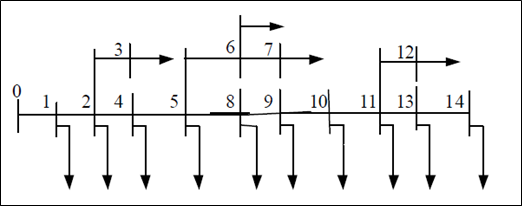
\includegraphics[width=0.85\linewidth]{figs/VR1.png}
\caption[One line diagram of a radial feeder]{One line diagram of a radial feeder.\cite{VR1}}
\label{fig:VR1}
\end{figure}

\begin{figure}[!h]
\centering
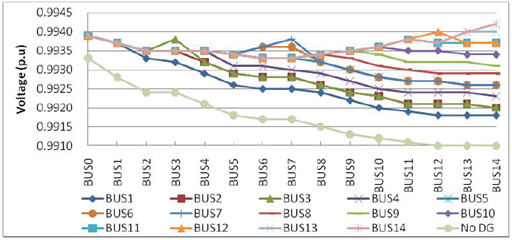
\includegraphics[width=0.85\linewidth]{figs/VR2.png}
\caption[Node voltage of PV accessing at different positions]{Node voltage of PV accessing at different positions.\cite{VR1}}
\label{fig:VR2}
\end{figure}

In addition to the change in the line voltage distribution, the presence of a variable DG in the system can cause a disturbance in the system voltage. Fig. \ref{fig:VR3} shows the load of a substation with and without a variable DG \cite{GKA11}. The variable DG, in this case, is a PV plant. In the figure, the normal demand on the substation is in black, and the demand with the presence of variable DG is in red. It can be seen that the red profile has a very irregular pattern. This voltage fluctuation can cause increased operation of the voltage regulation devices (OLTC, SCB and SVR). As these are mechanical devices, increased operations can decrease their life expectancy.
 
\begin{figure}[!h]
\centering
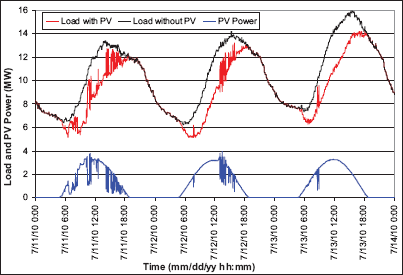
\includegraphics[width=0.7\linewidth]{figs/VR3.png}
\caption[Substation load with and without DG.]{Substation load with and without DG \cite{GKA11}.}
\label{fig:VR3}
\end{figure}
 

Fig. \ref{fig:VR4} shows the normal switching profile of a substation step voltage regulator without PV and Fig. \ref{fig:VR5} shows the switching profile with PV. As it can be seen from the figures, the presence of the variable DG caused much more switching operations. Moreover, DG near loads may increase the voltage in that zone beyond the limits set by standards. This increase in voltage may not trigger the voltage regulation devices as the nodes the devices are monitoring can stay within limits. Therefore, the controls of the devices may need to be upgraded as DG penetration in the grid increases \cite{IEE13}. These impacts can increase costs due to tear and wear in switching devices, decreases equipment life due to over-voltage and need for more power factor correction equipment. 

\begin{figure}[!h]
\centering
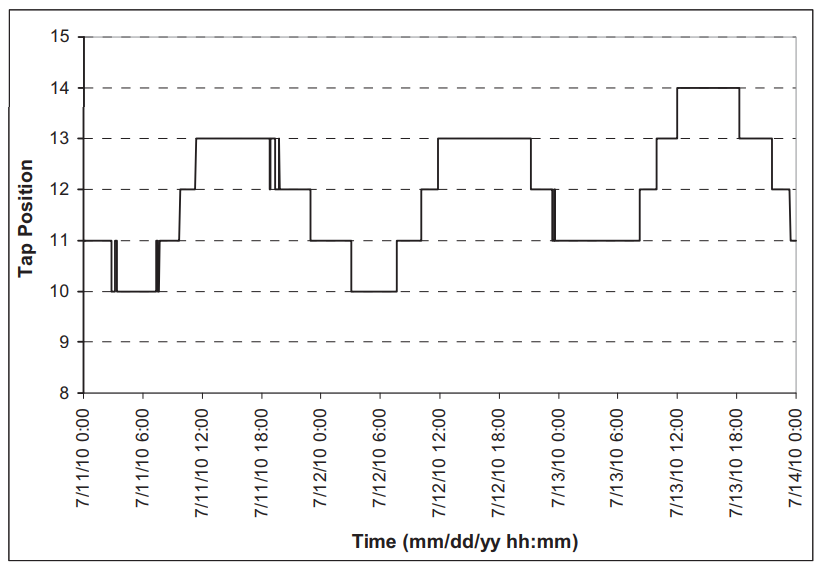
\includegraphics[width=0.85\linewidth]{figs/VR4.png}
\caption[Substation transformer tap changer position without DG]{Substation transformer tap changer position without DG \cite{GKA11}.}
\label{fig:VR4}
\end{figure}
 
 \begin{figure}[!h]
\centering
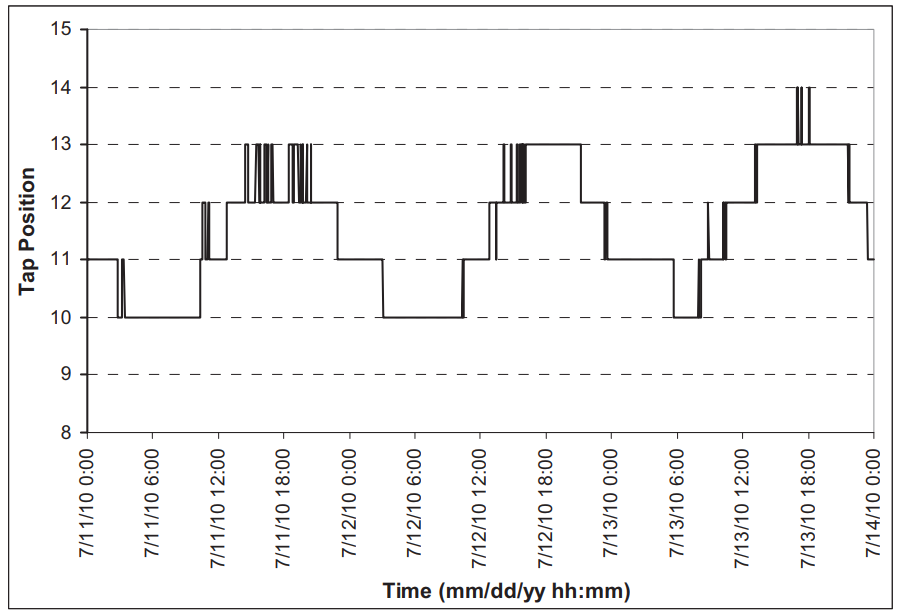
\includegraphics[width=0.85\linewidth]{figs/VR5.png}
\caption[Substation transformer tap changer position with DG.]{Substation transformer tap changer position with DG \cite{GKA11}.}
\label{fig:VR5}
\end{figure}

\subsubsection{System protection impacts}
The protection system of the distribution grid has been designed for unidirectional power flow. The integration of DG will require upgrading the protection system for better protection coordination. Usually, distribution systems employ protection schemes that consist of fuses, circuit breakers, sectionalizes, and automatic restoration devices that are coordinated in the load direction to operate with a minimum number of customers affected \cite{PRO1}. This coordination does not account for the integration of DG in the system. The integration of DG introduces more sources in the feeder to contribute to the fault current. Depending on the fault location, rating of DG and protection system installed, many problems could arise. Some of the possible problems are listed below.
\begin{enumerate}
    \item Fault level modification
    \item Blinding of Protection
    \item Sympathetic tripping
    \item Reduction in reach of distance relay
    \item Sensitivity reduction of high impedance fault detection
\end{enumerate}
Detailed analysis of the problems can be found in \cite{PRO2}.




\section{ADMS (Advanced Distribution Management System)}
From the previous discussion, it is evident that increased DER penetration is bringing some complex problems to be solved. To combat these emerging issues, new technology is being added to the aging infrastructure of the traditional power grid. These new technologies are known as "smart grid" technologies. The future evolving grid or “smart grid” has to incorporate information technology, communication technology and advanced control with power engineering. Another major aspect of the smart grid is control automation. The smart grid has to be self -healing and capable of maintaining system stability in case of system change and anomalies. Moreover, the grid of the future has to enable its stakeholders to realize new ways of performing energy transactions across the system while making sure it is financially viable and beneficial for both parties \cite{SG1}. To maximize the utilization of these new resources and data available, a proper management system is required. The concept of ADMS (advanced distribution management system) is introduced to handle this task. The concept of ADMS is still an evolving topic, and different sources define the components present in an ADMS system differently. However, irrespective of the internal architecture there are three major functions a modern ADMS system should be able to perform \cite{ADMS_1}.
\begin{itemize}
    \item Monitor and operate: An ADMS system should be capable of wide-area monitoring and operations. Utilities use SCADA systems to monitor the state of the grid from a central location. SCADA provides the current status of different protection systems, alarms and metering devices to aid the operator in system operation.
    \item Analyze and Optimize: Analysis and optimization are done using the distribution network applications included with the ADMS. The included applications vary between different ADMS providers. The main purpose here is to optimize the use of available resources without jeopardizing system stability.
    \item Track and Restore: With the integration of DERs and introduction of reverse power flow, the fault characteristics of a distribution grid has changed drastically. Proper identification of fault location very complex problem. ADMS solutions provide different components like outage management system, auto system restoration system, fault identification system, etc. to aid the utilities in fault detection and system restoration.
\end{itemize}
As the ADMS is an evolving technology, the ADMS architecture is defined differently by various sources. Fig. \ref{fig:ADMS_ARCH} shows the ADMS architecture proposed by the United States department of energy. The shaded region represents the sections which are still being actively developed and researched. Integrating these aspects with the existing management system is the major challenge of designing a modern ADMS system. Short descriptions of the different components of the ADMS architecture proposed by the United States department of energy are given below \cite{ADMS_2}:

\begin{figure}[!h]
\centering
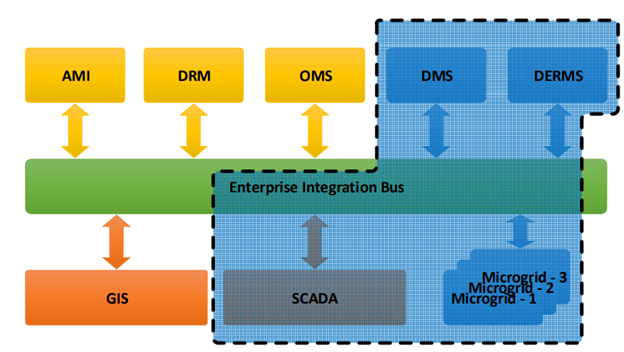
\includegraphics[width=0.85\linewidth]{figs/ADMS_ARCH.png}
\caption[ADMS architecture]{ADMS architecture. \cite{ADMS_2}}
\label{fig:ADMS_ARCH}
\end{figure}

 \begin{itemize}
     \item \textbf{AMI:} AMI represents the advanced metering infrastructure. The AMI is responsible for aggregating different measured data and sending it to the utility.
     \item \textbf{DRM:} DRM stands for dispatchable resource management. It chooses the most cost-effective way to modulate the traditional dispatchable resources to meet the current demand.
     \item \textbf{OMS:} The Outage Management System is in charge of managing the process of restoration after an outage has occurred in the grid. It is in charge of detecting incidents and automatically reconfiguring the network to have the least outage possible. It also deals with customer calls and crew management to restore service.
     \item \textbf{GIS:} A geographical information system (GIS) lets the utility analyze, interpret and visualize data based on geographical location. This helps the operators in real-time monitoring of the system. It also helps the operators to understand patterns and trends in the system.
     \item \textbf{SCADA:} The purpose of SCADA (supervisory control and data acquisition) is to monitor and control the system based on the data collected from different sources. SCADA is used for high-level supervision and management.
     \item \textbf{DMS:} DMS stands for Distribution Management System. This is used for managing different resources at the distribution level.
     \item \textbf{DERMS:} DERMS stands for Distributed Energy Resource Management System. DERMS work in conjunction with the DMS to ensure the efficient use of DERs in the distribution system. It can be viewed as a subsystem of the DMS in charge of DERs.
     \item \textbf{Microgrid:} Microgrids are entities capable of operating self-sufficiently with or without grid connection. The utility or another third party can own microgrids. The microgrids can be operated as a self-sufficient zone in times of high demand and faults.
 \end{itemize}

\subsection{DERMS (Distributed Energy Resource Management System)}
As this report focuses on components of DERMS, this concept is explained in more detail. The conventional power grid had an unpredictable and varying load profile. To counter this, the traditional grid used the dispatchability of traditional power plants and spinning reserves to maintain reliable power flow. It is also clear from the discussions thus far that the integration of distributed generation resources in the distribution system is increasing rapidly. As variable DG integration increases in the grid, the unpredictability of the grid rises drastically. The traditional approach of keeping spinning reserves are not only expensive but also inefficient to deal with this modern varying grid. Storage technology can play a crucial role in decreasing the variability of the grid \cite{USD13}. With recent advances in energy storage, utilities are considering deploying energy storage rated from 2kWh to 50 MWh in the distribution level \cite{Cle12}. Medium to small scale energy storage deployed near the consumer end lets the utilities provide better voltage control, renewable integration and reduced distribution losses while providing them the means to absorb fluctuation in prices and load. Moreover, with real-time pricing, the consumer can optimize the use of their energy storage and minimize electricity cost by taking advantage of the fluctuating price \cite{BPR11,PMv13,ASB17}.
Optimizing the use of energy resources can lead to a lower cost. However, grid voltage stability and constraints cannot be compromised to gain the optimal solution. Integration of DGs produce challenges for maintaining the system voltage stability. Another major concern is the new complexities that arise in properly protecting the system. The traditional protection schemes are not adequate in maintaining optimal system protection. To manage these new DERs at the distribution level, the concept of DERMS (Distributed Energy Resource Management System) has been introduced. Fig. \ref{fig:DERMS_ARCH} shows functions of a DERMS system. 

\begin{figure}[!h]
\centering
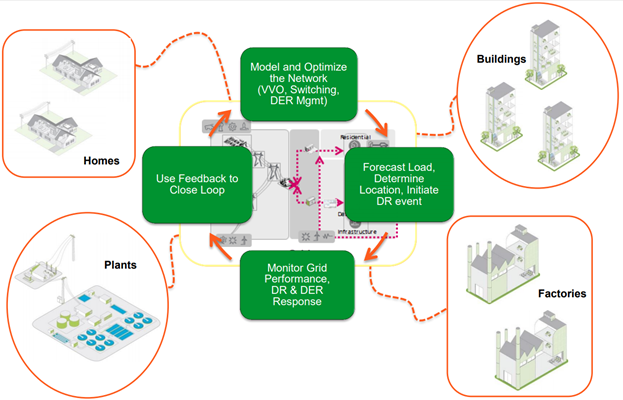
\includegraphics[width=0.85\linewidth]{figs/DERMS_ARCH.png}
\caption[Functions of DERMS.]{Functions of DERMS. \cite{DERMS_1}}
\label{fig:DERMS_ARCH}
\end{figure}

As seen in Fig. \ref{fig:DERMS_ARCH} the DERMS system achieves it's purpose by following a certain pattern. These functionalities are described below

\begin{itemize}
    \item Model and Optimize the network: This process uses the current system measurements and other additional available data to determine the current status of the system from a system model. After the system status is estimated, the estimation is used in optimizing different aspects of the system. Some common aspects are VVO (volt var optimization), network switching and DER management. The purpose of the optimization is to ensure minimum resource use without violating any system constraints.
    
    \item Forecast: With the addition of energy storing devices and volatile fast changing generation, proper forecasting of the system status has become an effective tool. The forecasts can provide an idea about the future load, DG availability and price. These information, in turn, can be used to optimize the system not only based on current status but also the probable future. This adds a whole new dimension to optimizing DERs and the best approach to forecasting and optimization based on forecasts are still a topic requiring much research.
    
    \item Monitor: The addition of DERs into the grid has introduced many new possibilities in the grid. But this does not come without demerits. The introduction of inverters and reverse power flow means that more monitoring devices are required to monitor the grid effectively. To tackle these issues, smart meters and PMUs (phasor measurement units) are being added to the distribution grid \cite{DPMU1}. But these devices are costly. To monitor the distribution grid using such devices is a vital task of DERMs. The most effective way to monitor the distribution grid using such devices is a topic of much interest.
    
    \item Feedback: The feedback part of the DERMs operation loop is mostly based on communication. After collecting the system status data, the feedback is responsible for providing it to the model and optimize the portion of the DERMs loop. This process can be a combination of wired and wireless communication.
\end{itemize}

From the discussion thus far it can be concluded that the DERMs system is in place to help both the utility and consumer optimize the use of the new DERs being integrated into the power system while maintaining system stability. The problems the DERMs faces can be divided into three main categories:
\begin{enumerate}
    \item Voltage control
    \item Optimum energy management
    \item Power system protection
\end{enumerate}

This research focuses mostly on the Voltage control and Optimum energy management aspects of DERMS. In the next chapter, the state of the art research on these categories is presented and the research gaps in the area are discussed.

\section{Motivation}
\subsection{Requirement for Coordinated Voltage Regulation with Increasing DER Penetration}
From the discussion so far, it is evident that the energy industry is rapidly approaching a significant penetration of distributed generation (DG) in the distribution system. This higher penetration of distributed energy resources (DERs) has introduced reverse power flow in the system. The traditional voltage regulation devices only consider unidirectional power flow and operate based on the consideration that the voltage down the line will decrease depending on the line impedance. However, this assumption is not valid with distributed generation as they can change the voltage of a node by supplying or absorbing reactive power. The uncertainty of the distributed wind and solar renewable resources can also cause traditional voltage regulation devices to operate more than necessary \cite{int1}. This results in faster degradation of the mechanical components of the traditional regulation devices. Also, the current response time for the traditional regulation devices is in the range of minutes. With fast changing DGs on the system, this may lead to over voltage or under voltage situations occur for several minutes throughout the day. On the other hand, the smart inverters used to interface DERs with the grid can be used in voltage regulation. Additionally, advanced metering architecture (AMI) and smart meters can provide a lot more data regarding the system status. How to efficiently use this data to optimize the use of traditional voltage regulation devices as well as the smart inverters present in the grid is still a contemporary research topic without a clear answer. All of these are the motivating factors behind the coordinated voltage control approach developed.

% With the rise of technology such as smart grid, advanced metering infrastructure (AMI) and phasor measurement units (PMUs), a lot more data regarding the system status is available. How to efficiently use this data to optimize the voltage control coordination is still a contemporary research topic. In most of the current literature, this problem is addressed as an optimum power flow problem or a mixed integer optimization problem \cite{int2}. But both these approaches usually propose methods which are very computationally intensive and time consuming. For example, in \cite{LR5,LR1,LR2,LR3}, researchers describe various methods to coordinate voltage control using the DG and traditional voltage regulation devices. But the control cycles in these methods are in the range of minutes to an hour \cite{LR4}. This makes them unfavorable for controlling the voltage in a distribution grid containing fast responding DGs. 

\subsection{Requirement for Energy Management with Increasing DER Penetration}
In the last few years, there has been significant growth in grid-connected distributed energy resources (DERs) leading to an increased deployment of distributed generation (DG) and recently more distributed storage (DS) systems. Companies have started to heavily invest in the competitive energy storage system market by taking advantage of the decreasing costs of energy storage. Although a significant amount of DG and DS are being added to the distribution grid, need to improve their control systems for seamless integration to the grid is still there. In the US, most DG and DS systems are deployed to either help reduce the metered load through net-metering programs or to sell power to the utility through power purchase agreements (PPAs). The potential of DG combined with DS is not fully utilized under these pricing schemes due to the lack of proper control schemes \cite{CONF_1}. In order to maximize the use of available DERs, a state-of-the-art energy management solution is a necessity for our future smart grid. Such an energy management solution will be able to dynamically optimize the use of all the available energy resources, with the objective of serving the load in the most economical and safe way possible. This will benefit both utility companies and regular consumers. Due to the constraints and intermittent nature of some DG systems, such as wind and solar, the optimum management of DS combined with a DG is a difficult problem to solve. All of these factors are the motivation behind the energy management approach developed.

% The most common approaches found in the current literature are as follows. Some researchers formulate the problem as a linear programming (LP) or mixed integer linear programming (MILP) model \cite{lp73, lp74, lp75}. Authors in \cite{pso80, pso81} present an energy management solution based on particle swarm optimization for a microgrid containing wind turbines and energy storage (ES) system. Other researchers propose crow-search and ant colony optimization models to solve the energy management problem for local microgrids as seen in \cite{csa87} and \cite{aco84}. There has also been model predictive control (MPC) based approaches for managing ES in microgrid settings as seen in \cite{energymanajaboulay,mpcmorstyn}.  Researchers in \cite{ga76, ga77} have also proposed genetic algorithm based solutions to optimize the ES operation in a microgrid. One clear disadvantage of these proposed models is that most of these approaches only consider the current status of the system and ignore some critical factors like energy tariff, forecasted load, and forecasted generation profiles.  These information can be used to find an optimum solution based on both current and probable future states of the system as opposed to a solution relying only on the currently available data. Off-line day ahead planning models have also been proposed in the literature. In these methods, available predicted data is used to optimize the scheduling of the ES based on Monte Carlo simulations \cite{6872821,7010943,6839110}. These solutions are very computationally intensive and require a lot of time for planning the day ahead. The computational complexity makes them unsuitable for real-time implementation also, as they are based on off-line calculations and rely vastly on the accuracy of the predictions.

% From the discussion thus far, it is evident that there is a need for a real-time ESM solution that can optimize the long-term operating costs of a system containing DG and an energy storage (ES) system. 

%\section{Research Gap and Contributions}


% \subsection{Effect on voltage Regulation Devices}

% \section{Energy Management Under Changing price}






\chapter{Literature review, Research Gap and Contributions}
From the discussion in chapter \ref{TH_intro}, it is evident that with the integration of DERs in the grid, several new challenges are coming into light. To help in the integration of DERs and combat these challenges, ADMS and DERMS are being developed. Two significant components of DERMS are voltage regulation and energy management. This chapter focuses on the state of the art research on these two topics. Analysis of research gaps in the areas and novel contribution of the research are also presented. 
\section{Voltage Regulation}
As mentioned in chapter \ref{TH_intro}, voltage regulation is one of the primary challenges to be overcome in order to have a high penetration of DERs in the grid. Currently, there are two types of regulation devices available in the system. The first type is the traditional regulation devices (on load tap changers, switched capacitor banks, step voltage regulators) and the other types are power electronics based regulation devices (DG inverters and distribution static VAR compensators). There needs to be an optimum operation of both to reliably and cost-effectively maintain the voltage at all the nodes of the system. In literature, this problem is defined in two ways. It can be defined as an Optimum voltage regulation problem, or it can be defined as an optimum reactive power dispatch problem. Many alternative methods with different controllable components have been discussed in the literature to solve the problem. The following is a brief discussion of the controllable components which may be used to solve the problem \cite{VC_1}. 
\begin{itemize}
    \item \textbf{Generation curtailment during low demand:} The DGs generation may be curtailed during low demand periods to maintain the system voltage. This would be harmful to the DG owner because the DGs cannot operate in peak condition.
    \item \textbf{Reactive power control (VAR compensation) by reactive compensator:} Reactive VAR compensators placed at strategic points of the system can be used to absorb or inject reactive power.  
    \item \textbf{Area based OLTC (on load tap changer) coordinated voltage control:} The OLTC at the substation can be controlled to maintain voltage.
    \item \textbf{Inverters at DG sites:} The inverters of the DGs can be used similarly to the VAR compensators to inject reactive power or absorb reactive power as needed.
    \item \textbf{Energy storage:} If there are energy storage in the system, their charging and discharging operations can be controlled to maintain system voltage.
\end{itemize}

Control methodologies which take into account all the components are still a topic of interest. Some of the recent research on the topic are stated below.

% \subsection{Centralized Control}
% In this control strategy, every component of the distribution system is controlled from a centralized controller. Proper implementation of these methods requires a robust communication network in the distribution system. The centralized control methods considered here focus on control algorithms that make use of the DG inverters to maintain global voltage. 

An objective function to minimize active power loss in distribution network has been considered in \cite{CE_VC_1}. The researchers here use particle swarm optimization with historical data to plan the optimum power flow every 15 minutes. Although this algorithm is shown to plan and coordinate voltage control efficiently this algorithm requires historical data and a good prediction. Also the 15 minutes time interval might be too long to respond to voltage violations effectively. Researchers in \cite{CE_VC_2} focuses on reactive power control with an objective of minimizing voltage deviation at each bus according to a reference voltage. Here the researchers optimize the total system at fixed time intervals to minimize voltage deviation. This approach has similar drawbacks as \cite{CE_VC_1}. Using predictive data to optimize future status of the system may cause less voltage violations but the long and complex computation necessary for the method makes it unsuitable for quickly responding to voltage violations. 
%In \cite{CE_VC_3}, the distribution network has been divided into different subsections to reduce the optimization complexity.
In \cite{CE_VC_4} tap operation and system losses in radial distribution network were minimized by coordinating OLTCs and SVCs (static VAR compensators). In this approach the researchers relaxed the mixed integer nonlinear programming to a continuous non linear programming problem and solved the relaxed problem. The researchers here do not consider the  reactive power generation capabilities of the inverter interfaced DGs.
In \cite{NLR_1}, researchers propose a model predictive control (MPC) based technique where they curtail the DG generation based on the distribution network operator requirements. The researchers assume Voltage magnitude and angle measurements are available to the algorithm. The researchers state that the MPC can be formulated as a quadratic program and solved using commercial solvers.
In \cite{NLR_2} researchers propose a decentralized control scheme where they divide the distribution system into different control zones based on the position of voltage regulators. Each control zone is controlled independently of each other. The coordinated voltage regulation problem is formulated as a minimization problem in this case as well, and the optimum tap position of the voltage regulators are determined using big-bang crunch optimization. The researchers here consider a 15-minute control horizon and assume real-time measurement from the system is available.
The researchers in \cite{NLR_3} propose a coordinated voltage control scheme based on data collected from the distribution system phasor measurement unit (DPMU). Here the researchers propose using a reduced system model by representing the nodes between DPMUs as equivalent $\pi$ or T  lines. Then a rule-based control methodology is used to coordinate voltage regulation.  
Researchers in \cite{NLR_4} present another rule-based approach where they consider a DC microgrid, as well as traditional regulation, devised added to the grid. The researchers validated their algorithm using power hardware in the loop real-time simulation. 
Researchers in \cite{NLR_5} use MPC based approach to control the voltage in a distribution grid by running two different MPCs in parallel in different time scale. The traditional regulation devices in conjunction with the available DG inverters in the system are controlled using a complex MPC formulation. In between the time it takes to solve the complex MPC problem the results of the previous solution is used to optimize the use of available fast responding DERs in the grid. This allows for a fast time scale control to optimize the system in between slower time scale control actions. The slow time scale control action is performed every 60 minutes and the fast time scale control action is performed every minute. The researchers assume system data is available from SCADA in this case. The method mentioned here uses mixed integer programming, and the convergence of the problem depends on the giving it a proper starting criterion. Which means if the initial conditions are far from the actual conduit of the grid the algorithm will not converge. This makes the approach vulnerable to failure from bad data.
Researchers in \cite{NLR_6} use optimum power flow to solve the voltage regulation problem. They use a distributed control approach called fast distributed optimal reactive power flow algorithm. The algorithm uses local controllers or agents at DG nodes which operate based on information available from neighboring nodes. The formulation only deals with reactive power supplied by DG inverters and do not consider coordinating with traditional regulation devices. 
In \cite{NLR_7}, a control strategy to coordinate the traditional regulation devices with grid-connected microgrid is proposed. The test system used in this study is a four bus system with three buses containing microgrids. The problem is formulated as an MPC and solved using a cooperative distributed MPC strategy. They show coordination between the connected microgrids, capacitor banks, and OLTC. The microgrids are able to maintain the required voltage at their point of common coupling (PCC).
In \cite{NLR_8}, researchers propose a control strategy based on a hybrid approach where local controllers maintain voltage using volt-var control. Then a centralized controller further refines the local controls based on an MPC formulation. They assume system data of all the nodes are available. This allows faster local correction in seconds while the global centralized MPC refines the solution every tens of seconds.
Researchers in \cite{NLR_9} propose a multi-objective pareto front optimization based technique to optimize the voltage regulation. They use genetic algorithm (GA) to determine a set of non dominated solutions offline. This step can take hours to perform. Then knowledge based local search (KBLS) is done on the reduced solution space achieved from the GA to get the solution based on current objective. If current objective is lowest cost of operation the KBLS looks for the solution with the least cost. if the current objective is fast voltage recovery then the KBLS will look for a solution that is within the regulation limits. This allows for creating reduced solution spaces offline and then the use of KBLS online to find the solution based on system operator needs. The researcher here show numerical simulation to verify the proposed method.
In \cite{NLR_10} researchers propose a coordinated control scheme that take into account both fast changing and slow changing operations. The researchers here propose using model reduction of the distribution grid. Here they represent the distribution grid elements between regulation devices and VSC connected DGs into equivalent circuit models. Then the reduced model is used to verify the effectiveness of the optimization. The researchers here use a sensitivity analysis based technique to coordinate the system voltage.



%IN \cite{CE_VC_5}, the day ahead prediction of DGs were used to aid in the regulation method. Another control strategy utilizing energy storage systems and OLTCS is proposed in \cite{CE_VC_7}.

% % A centralized control strategy can provide the best performance possible, but it may not be the best solution for the future grid for the following reasons \cite{VC_1}:
% % \begin{itemize}
% %     \item They require significant investment in communication assets.
% %     \item A large number of small scale devices need to be controlled.
% %     \item There is an increased amount of uncertainty due to faults, electric vehicles, storage units, dynamic loads, variable DGs, restoration, reconfiguration etc.
% %     \item Increased computation complexity due to a large number of variables.
% %     \item Does not incorporate plug and play capabilities.
% % \end{itemize}

% \subsection{Decentralized and Distributed Control}
% Decentralized and distributed control schemes do not have a centralized hub where the control actions are calculated. They consist of multiple controllers which communicate with each other to maintain system stability \cite{DB_VC_1}.  Different decentralized and distributed control schemes are briefly discussed below.

% \begin{itemize}
%     \item \textbf{Distributed optimization method:} The optimum voltage control problem can be formulated as a non-convex optimal power flow problem. In these methods, some form of convex relaxation is applied to make the problem convex. Then the centralized convex problem is decomposed to and solved by distributed algorithms \cite{Kyrue}. References  \cite{KUt17,BAR16,BAR161,WZh16} are some of the recent literature using various distributed optimization methods to solve the voltage regulation problem.
%     \item \textbf{Decentralized Methods:} In the decentralized method, each area solves its own voltage regulation problem and the solution only affects that area. Both heuristic methods and optimization methods may be used to solve the problems \cite{Kyrue}. \cite{MChss,MBa,XZh16,MNa16,LRe15,EDass} are some recent publications on this method.
%     \item \textbf{Distributed Cooperation:} In this scheme, the secondary centralized control interacts with autonomous primary control. This results in a secondary control scheme that substitutes local control \cite{Kyrue}. References \cite{ABi13,FGu15,SAn13,QSh14} are some modern research on this topic.
%     \item \textbf{Distributed Adaptive Control:} These methods monitor their performance and self-tunes its input value rather than maintaining a reference value. In \cite{ABi14} the adaptive secondary voltage control is formulated as a tracking synchronization problem. Neural networks were used to model the non-linear inverter dynamics \cite{Kyrue}.
%     \item \textbf{Distributed Model Predictive Control:} In this method, the controllers predict their state over a finite time-horizon by gathering information from their neighbors and using the model of the system. In \cite{GLoss} model predictive control is used to minimize the voltage deviation until all the voltages synchronize to a reference value \cite{Kyrue}.
%     \item \textbf{Decision Making:} In this method, when there is a conflict between multiple objectives a decision maker is used to identify the solution \cite{Kyrue}. Expert-based decision makers are incorporated in smart agents in \cite{HEF12, HEF13}. The agents communicate using a contract net protocol option. The controllers in \cite{MEC13} exchange their constraints to solve a dynamic optimal dispatch problem.
%     \item \textbf{Hybrid Methods:} In this case, the distributed control takes over when the local control fails to maintain the system voltage \cite{Kyrue}. Reference \cite{GMo13,YWa16} uses consensus algorithms for distributed control after local control fails. Reference \cite{DRe13} does active curtailment of DG units. In \cite{BAR13} the distributed control requests reactive power compensation from neighboring zones if voltage imbalance cannot be mitigated.
% \end{itemize}
% An overview of the advantages and disadvantages of the methods mentioned is given in Fig. \ref{fig:DIS_CVC}.
% \begin{figure}[!h]
% \centering
% 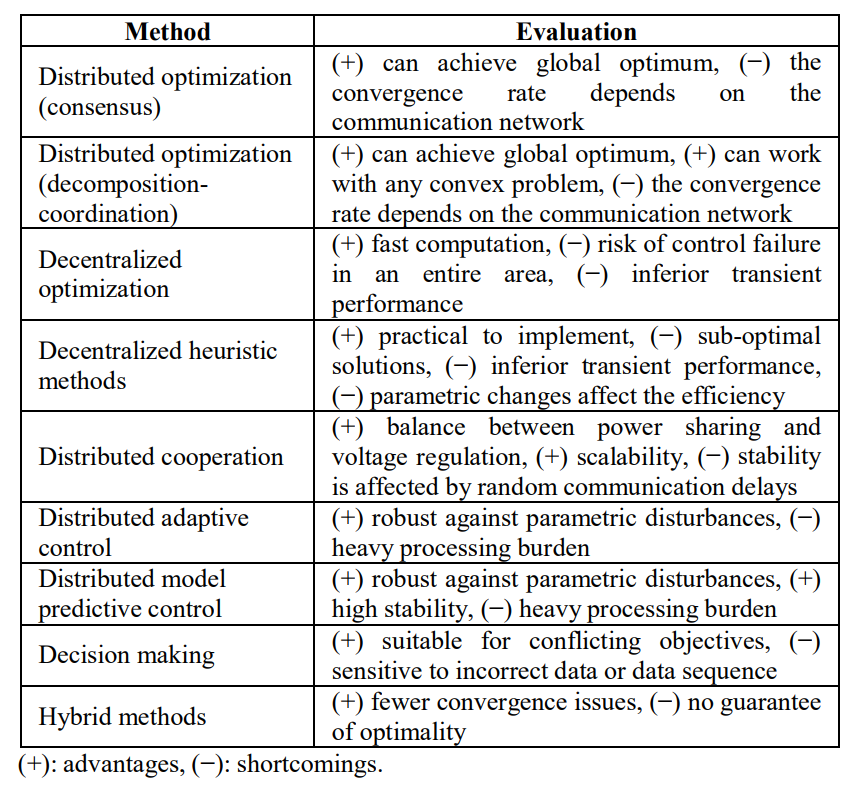
\includegraphics[width=0.85\linewidth]{figs/DIS_CVC.png}
% \caption[Evaluation of mentioned methods]{Evaluation of mentioned methods \cite{Kyrue}}
% \label{fig:DIS_CVC}
% \end{figure}

\section{Energy Management}
With real-time pricing and variability of DGs, energy management can play a vital role to decrease the cost of energy. The goal of a modern energy management system would be to optimize the use of energy storage not only based on the current state of the system but also based on the probable future states. The energy management algorithms which deal with both variable DGs and real-time pricing can be divided into two main categories, offline and real-time algorithms \cite{Wen17}. 
\subsection{Offline Algorithms}
The offline optimization algorithms usually optimize energy for a predetermined time horizon based on prediction data. Researchers in \cite{ACh13} use neural network combined with linear programming based multi-objective optimization to optimize the use of several DERs in a microgrid. They also use fuzzy logic based expert system to schedule the use of energy storage. Fig. \ref{fig:OFF_1} shows the microgrid architecture under consideration in this research. The researchers use 24-hour ahead PV forecasting and 1-hour ahead wind energy forecasting to optimize the use of the resources. Although this approach guarantees global optimization, huge computation power is necessary to scale this for larger systems. Also, the optimality of the solution is based on considering perfect prediction.

\begin{figure}[!h]
\centering
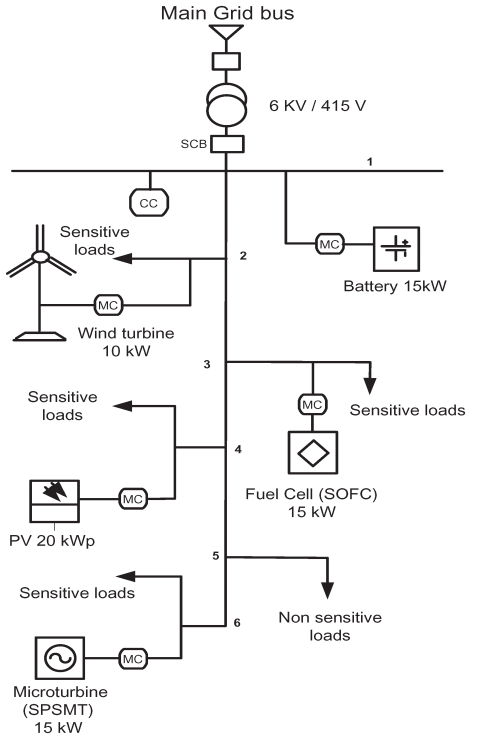
\includegraphics[width=0.5\linewidth, angle = 90]{figs/OFF_1.png}
\caption[Microgrid architecture under consideration]{Microgrid architecture under consideration in \cite{ACh13}.}
\label{fig:OFF_1}
\end{figure}

Researchers in \cite{AKh14} propose a microgrid optimization problem which runs the microgrid in islanded mode if enough generation is available and connects to the grid if enough generation is not available in the microgrid or the cost of using the local DERs becomes higher than the grid cost. Fig. \ref{fig:OFF_2}  shows the flowchart of the proposed scheduling model. The problem is defined in two parts. A grid-connected operation master problem a subproblem for islanded operation. First, the master problem determines the optimal scheduling of the available resources with the grid. Then the schedule is passed down to the subproblem to determine the feasibility of the microgrid operation. If the microgrid does not have the capability to pertain to the schedule, it cuts back the deficiencies from the schedule and returns the new schedule to the main problem.  The proposed method schedules the microgrid operation intentional islanding operations a day ahead based on predicted data. This makes the method highly reliant on perfect prediction. \cite{WSh15} presents an off-line method that takes into account the underlying structure of the grid. The researchers propose a scheduling method based on optimum power flow to ensure none of the scheduled states violate system constraints. The system is optimally scheduled taking the help of both a global controller and locally placed distributed controllers. The methods mentioned thus far show significant saving under ideal conditions. However, the reliability on perfect prediction and non-scalable nature of some of the solutions make them impractical for implementation on the actual grid.

\begin{figure}[!h]
\centering
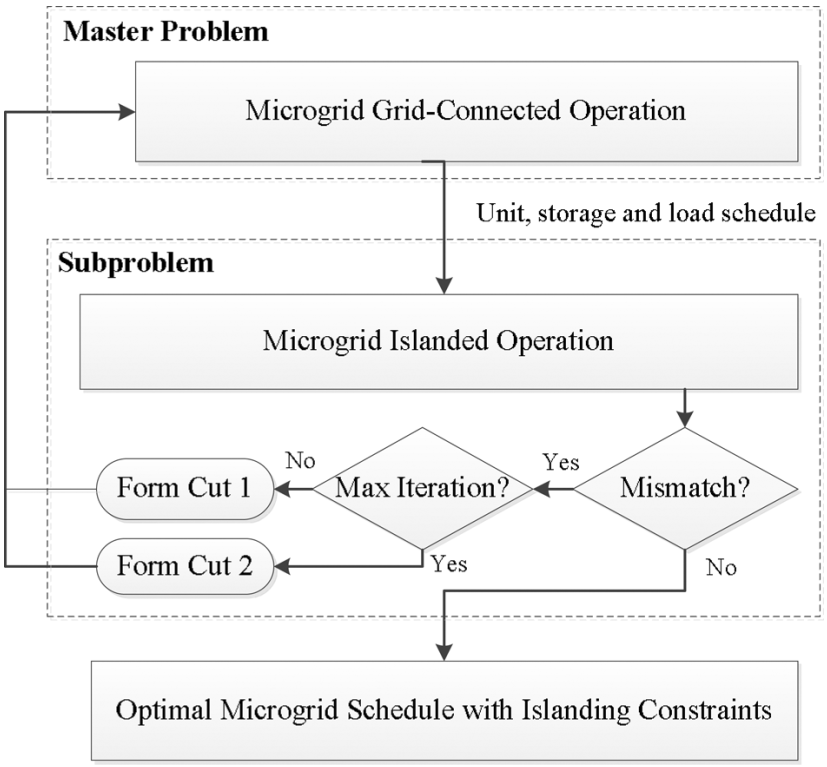
\includegraphics[width=0.5\linewidth]{figs/OFF_2.png}
\caption[Proposed scheduling model]{Proposed scheduling model  in \cite{AKh14}.}
\label{fig:OFF_2}
\end{figure}

To solve the problem of reliance on perfect prediction some offline algorithms, try to model the uncertainties in day-ahead scheduling and try to develop optimum schedules taking into account the probable uncertainties.
\cite{Has17} uses mixed integer linear programming formulation of the day ahead scheduling of microgrids. The uncertainties are taken into account by calculating multiple solutions based on different predicted seniors. 
The authors in \cite{Yue16} formulate the optimization problem based on the worst case scenario. The solution method considers the most cost from the grid and the least benefits from using local DG resources. The uncertainty of the grid is expressed as set points in Taguchi’s orthogonal array. Then search strategy based on Taguchi’s orthogonal array is used to find the best possible solution cases. Using the worst case to formulate the problem makes the solution robust for all situations. Although this method provides a robust solution always taking into account, the worst scenario makes the solution suboptimal.
\cite{FFa15} uses the mixed inter programming formulation for optimizing the DERs. The uncertainties of the predicted data are taken into account by generating different schedules with risk-averse and risk-neutral options. The different scenarios are stochastically generated based on the risk-based prediction data available. The approach uses stochastic programming to generate the uncertainties as different scenarios. The number of scenarios required to adequately capture the uncertainties usually end up being very large. 

\subsection{Real-Time Algorithms}
There have been advances recently in designing real-time algorithms that optimize the long-term cost of the energy management system, taking into account the intermittent nature of the loads and DGs in the grid. \cite{RPa13} Proposes a real-time management process based on a rolling horizon strategy. The algorithm proposed solves a mixed integer linear programming problem in each interval to generate setpoints for the resources available. The researchers test the algorithm using a microgrid model consisting of a PV panel, diesel generator, wind turbine and energy storage system. Fig. \ref{fig:RT_1} shows a block diagram of the proposed method. As it can be seen from the diagram, the method takes into account historical data, current measurement and weather forecast in the optimization process. The system discussed has to solve a mixed integer linear program on every time interval. This process is computationally intensive and becomes exponentially more complex with the addition of more energy resources.
\begin{figure}[!h]
\centering
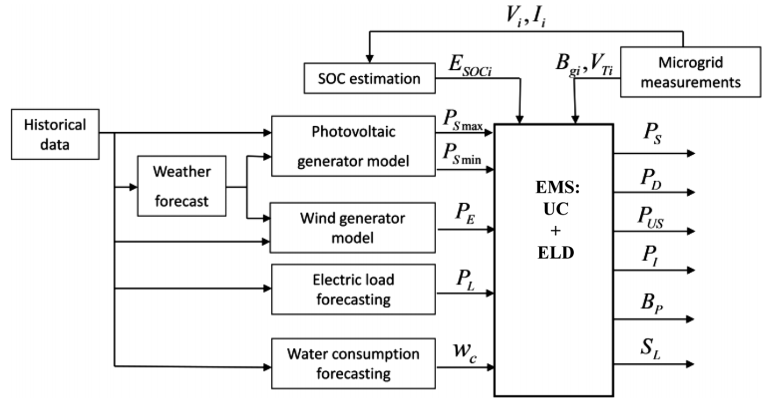
\includegraphics[width=0.85\linewidth]{figs/RT_1.png}
\caption[A block diagram of proposed energy management system]{A block diagram of proposed energy management system  \cite{RPa13}.}
\label{fig:RT_1}
\end{figure}

 Researchers in \cite{Sun14} use an aggregator to minimize the long-term cost of the grid. Figure 40 shows the top level schematic representation of the control architecture proposed. The solution used Lyapunov optimization to solve the energy management problem in real-time. The method proposed does not consider the actual architecture of the grid and optimizes considering all the components are connected to the same bus. This makes it impractical due to the actual grid having line constraints that cannot be violated.

\begin{figure}[!h]
\centering
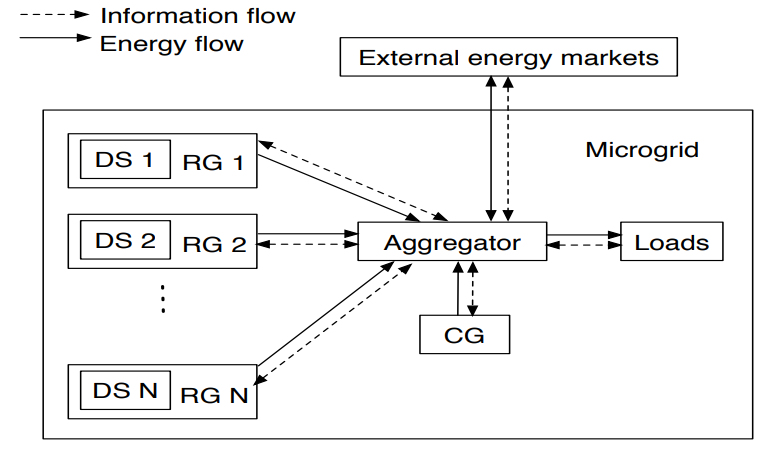
\includegraphics[width=0.5\linewidth]{figs/RT_2.png}
\caption[Schematic representation of solution method prepossessed]{Schematic representation of solution method prepossessed in \cite{Sun14}.}
\label{fig:RT_2}
\end{figure}

\cite{Men16} formulates the problem as a real-time one leader N-follower Stackelberg game and shows an efficient approach designed to optimize the system based on a demand response scheme. The optimization is performed by creating a virtual electricity trading market where the facility (leader) produces virtual prices of electricity and the resources (followers) compete to buy and sell electricity. The researchers show the existence of unique Stackelberg equilibrium for optimum use of each resource.

In \cite{Tia17}, researchers propose a multi-period AC optimal power flow taking into account the uncertainties of the solar and wind resources to ensure reliable solutions for the distribution system operators. Figure 41 shows the developed method in \cite{Tia17}. In the first stage, the algorithm contacts with all the available resources to determine the upper and lower bounds of generation throughout the next day. The upper and lower bounds of the different units are termed as flexibility in the paper. In the second stage, which is the real-time operation, the algorithm optimizes in real-time taking into account the flexibility of the available resources. 
 
\begin{figure}[!h]
\centering
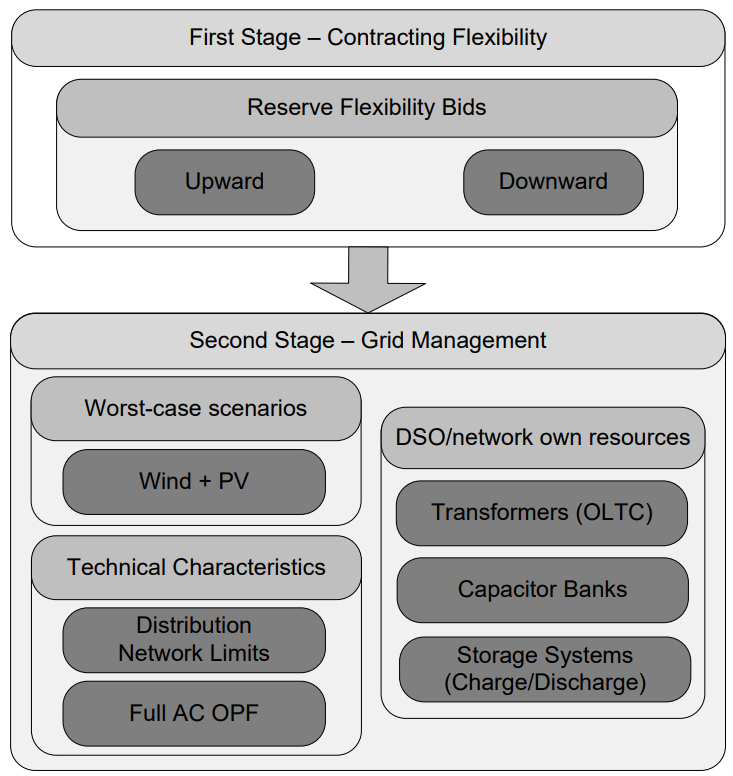
\includegraphics[width=0.4\linewidth]{figs/RT_3.png}
\caption[Methodology developed]{Methodology developed in \cite{Tia17}.}
\label{fig:RT_3}
\end{figure}

\cite{Wen17} proposes to solve the problem using an online energy management system in real-time using Lyapunov optimization taking into account the physical constraints of the system.
The drawbacks of these methods are that most of them do not take into account the actual distribution system architecture while formulating the problem. Only \cite{Wen17} considers system architecture while optimizing in real-time. However, a lack of prediction based elements makes these methods optimal for short term costs but suboptimal for properly optimizing long term operating cost.


\section{Research Gap}
From the discussion thus far, it is evident that there are still many research opportunities in the field of coordinated voltage control and real-time energy management of distribution grids containing DERs. Some of the research gaps in the literature are:

\subsection{Coordinated voltage control research gap}
The problem of coordinating the traditional regulation devices with the grid-connected DERs to regulate distribution system voltage is still being actively researched. There are novel solutions proposed, but they suffer from one or more of the limitations discussed below:
\begin{itemize}
    \item They consider that the voltage angle, magnitude, and real \& reactive power from all the nodes are available.
    \item They simplify the system based on the location of measurement devices which may lead to voltage violation inside the simplified sections.
    \item They only consider DERs or traditional voltage regulation devices to control the system voltage. Which loses the potential benefit of coordinating between DERs and traditional regulation devices.
    \item Some of the proposed solutions takes tens of seconds to minutes to determine the control action. This might not be fast enough response in systems with fast-changing DGs.
\end{itemize}

\subsection{Energy management research gap}

    
%     \item Real-time energy management research gap: With the increasing amount of variable DGs being added to the grid, it is becoming very difficult to have accurate long term prediction of grid status. The presently available solutions either use present grid status to do real-time control or use day ahead scheduling or use a mix of both to do energy management. There is still the need for an energy management scheme that can optimize system status in real-time with a continuously updating forecast. 
% \end{itemize}

\section{Contribution}
The efforts invested in the dissertation work at hand mainly aim towards the following:
 
\subsection{Development of coordinated voltage control algorithm}
A coordinated voltage control algorithm will be developed, which can make use of the reactive power generation capabilities of the inverter interfaced DERs and coordinate these resources with the existing traditional regulation devices. For this purpose, a solution methodology combining the Voltage Sensitivity Analysis \cite{Th_ali} and Electrical Distance Calculation \cite{Alvi3} concepts will be explored.

Major work under this task:
\begin{itemize}
    \item Design of proposed voltage control algorithm 
    \item Implementation of voltage control model in centralized or decentralized network typologies
    \item Compare performance of the proposed model with traditional voltage regulation scheme
\end{itemize}

\subsection{Development of real-time energy management system}
An energy management system that takes into account the physical system constraints while optimizing the use of available energy resources not only based on the current price but also based on the forecasted price will be developed. This part will be implemented by dividing the energy storage into separate states and creating a graph taking into account the system constraints. The solution of the energy management problem will be developed using a combination of the traditional optimal dispatch of generation solution, using the Linear programming model with DC power flow, with a graph search solution obtained from the utilization of the A* algorithm designed to find the optimal and most cost effective solution for dispatching available energy resources taking into account not only the present status of the system, but also the future forecasting values of the energy prices, load demand, and generation.
To accommodate the forecasted data into decision making. The energy storage (ES) capability of the system is divided into discrete states of charge (SOC). Then a graph is constructed to represent the states of charges with respect to time. Each edge of the graph will have a total cost. The total cost will be calculated, taking into account the economic dispatch of the resources available in the system. After the graph is constructed, A* search algorithm will be used to find the optimal path.

Major work under this task:
\begin{itemize}
    \item Design of proposed A* star algorithm model 
    \item Integration of forecasting information
    \item Compare performance of the proposed model with other available schemes.
\end{itemize}


At present, a coordinated voltage control algorithm has been developed and validated using off-line simulation. Currently, it is assumed that the algorithm has access to the system voltage magnitude and angles. Moreover, a real-time energy management algorithm to optimize the use of a single grid-connected energy storage has been developed. The algorithm has been validated using controller hardware in the loop simulation.

\chapter{Coordinated Voltage Control in Distribution
Systems with Distributed Generations} \label{CVC}
This chapter proposes a coordinated voltage control method that reduces the use of traditional voltage regulation devices and utilizes the reactive power generation capabilities of the DG inverters to regulate the distribution system voltage. The proposed algorithm enables cooperation between multiple DGs to control the system voltage. This ensures that the full potential of the DG inverters is utilized before using the traditional devices for voltage regulation. The proposed method also completes its control cycle within seconds which makes it suitable for distribution grids containing fast changing DGs. The proposed method has been validated using a distribution feeder model based on a real feeder. A phasor model of the system with the control algorithm was simulated in MATLAB\textsuperscript{\textregistered} Simulink\textsuperscript{\textregistered} using the Simscape Power Systems\textsuperscript{TM} toolbox for validation.


\section{Design of Control Algorithm}\label{sec:design}
The proposed algorithm makes use of two concepts in order to coordinate the voltage regulation between the nodes. They are:
\begin{itemize}
\item Voltage sensitivity analysis
\item Electrical distance calculation
\end{itemize}
\subsection{State Estimation}
\subsection{Voltage Sensitivity Analysis}
The aim of the voltage sensitivity analysis is to determine the effect on the voltage of a certain node due to reactive power injection at different nodes in the feeder. Equation (\ref{eq.Pf_equation}) represents the system power-flow equation.  Here ${\Delta Q}, {\Delta P}, {\Delta |V|}$ and ${\Delta \delta}$ represent the change in real power, reactive power, voltage magnitude and voltage angle of nodes. $J$ represents the system Jacobian matrix. The elements of $J$ are shown in (\ref{eq.J_equation}).
\begin{equation}\label{eq.Pf_equation}
\begin{bmatrix}
{\Delta P}\\ {\Delta Q}
\end{bmatrix} =J\begin{bmatrix}
{\Delta|V|} \\ {\Delta\delta}
\end{bmatrix}
\end{equation}  
Where,
\begin{equation}\label{eq.J_equation}
    J = \begin{bmatrix}
{J_{P|V|}} & {J_{P\delta}}\\ {J_{Q|V|}} & {J_{Q\delta}}
\end{bmatrix}
\end{equation}

Using the components of the system Jacobian matrix the $J_{VQ}$ and $J_{VP}$ matrices can be formulated using (\ref{eq.JVQ}) and (\ref{eq.JVP}).
\begin{equation}\label{eq.JVQ}
    {J_{VQ}} = {J_{Q|V|}}-{J_{Q\delta}}{J_{P\delta}}^{-1}{J_{P|V|}}
\end{equation}

\begin{equation}\label{eq.JVP}
    {J_{VP}}={J_{P|V|}}-{J_{P\delta}}{J_{Q\delta}}^{-1}{J_{Q|V|}}
\end{equation}

Using (\ref{eq.JVQ}) and (\ref{eq.JVP}) the total voltage sensitivity due to real and reactive power injected by a DG can be calculated using (\ref{eq.V_PQ}) \cite{Th_ali}. Here, $[\Delta|V|_{PQ}], [P_{PV}] $ and $[Q_{PV}]$ represent the total voltage change, real power injected by DG and reactive power injected by DG, respectively.

\begin{equation}\label{eq.V_PQ}
[\Delta|V|_{PQ}] ={ J_{VP}}^{-1} [P_{PV}]+{ J_{VQ}}^{-1} [Q_{PV}]
\end{equation}

Using the relation $[P_{PV}] = \frac{[Q_{PV}]}{\cos^{-1}(p.f)}$, equation (\ref{eq.V_PQ}) can be written as
\begin{equation}\label{eq.V_Q}
 [\Delta|V|_{PQ}] ={ J_{VP}}^{-1}\frac{[Q_{PV}]}{\cos^{-1}(p.f)} +{ J_{VQ}}^{-1} [Q_{PV}]
\end{equation}
From (\ref{eq.V_Q}) we can get
\begin{equation}\label{eq.Q_V}
 [\Delta|V|_{PQ}] =( \frac{J_{VP}^{-1}}{\cos^{-1}(p.f)} +{ J_{VQ}}^{-1}) [Q_{PV}]
\end{equation}
And finally from (\ref{eq.Q_V}) we can get
\begin{equation}\label{eq.PV_Q}
 [Q_{PV}] = J_{PVQ} [\Delta|V|_{PQ}] 
\end{equation}
where,
\begin{equation}
J_{PVQ} = ( \frac{J_{VP}^{-1}}{\cos^{-1}(p.f)} +{ J_{VQ}}^{-1})^{-1}
\end{equation}
 Equation (\ref{eq.PV_Q}) gives us the relation between total voltage sensitivity and reactive power injection. Here, '$p.f$' represents power factor.

\subsection{Electrical Distance Calculation}
Electrical distance is calculated in order to determine the relative impact on one node due to a change in another node. The electrical distances are calculated by determining $M_{sVQ}$ according to equation (\ref{MsQV}) \cite{int1}.

\begin{equation}\label{MsQV}
\begin{bmatrix}
M_{s\alpha}P & M_{s\alpha}Q \\ 
M_{sVP} & M_{sVQ} 
\end{bmatrix} = J^{-1}
\end{equation}
 Here, $J$ is the system jacobian matrix and $M_{s\alpha}P, M_{s\alpha}Q, M_{sVP}$ and $M_{sVQ}$  are the four elements of the inverse of the system jacobian matrix. Equation (\ref{MsVq_expan}) shows the elements of $M_{sVQ}$. \cite{int1}

\begin{equation}\label{MsVq_expan}
M_{sVQ} =
\begin{bmatrix}
\frac{\delta V_{s1}}{\delta Q_{s1}}  & \frac{\delta V_{s1}}{\delta Q_{s2}} & \cdots & \frac{\delta V_{s1}}{\delta Q_{sn}}\\

\frac{\delta V_{s2}}{\delta Q_{s1}}  & \frac{\delta V_{s2}}{\delta Q_{s2}} & \cdots & \frac{\delta V_{s2}}{\delta Q_{sn}}\\

\vdots & \vdots & \vdots & \vdots\\

\frac{\delta V_{sn}}{\delta Q_{s1}}  & \frac{\delta V_{sn}}{\delta Q_{s2}} & \cdots & \frac{\delta V_{sn}}{\delta Q_{sn}}\\ 
\end{bmatrix}
\end{equation}
 
Here $V_{sn}$ and $Q_{sn}$ represent the voltage and reactive power of the node $n$. The electrical distance $D_{sij}$ between the nodes $i$ and $j$ can be calculated using (\ref{ED}) \cite{int1}. 

\begin{equation}\label{ED}
D_{sij} = -\log (\mu_{sij} * \mu_{sji})
\end{equation}

Where,
\begin{equation}
\mu_{sij} =  \frac{\delta V_{si}}{\delta Q_{sj}} / \frac{\delta V_{sj}}{\delta Q_{sj}}
\end{equation}


\subsection{Singular value decomposition and pseudo inverse}

In case of a distribution system, the system Jacobian matrix $J$ is usually a sparse matrix due to the radial nature of distribution systems. Calculating the inverse of $J$ becomes problematic due to this property. For this reason, (\ref{eq.PV_Q}) and (\ref{ED}) are implemented by determining the pseudoinverse of $J$ using singular value decomposition. The system Jacobian matrix $J$ can factored into the expression shown in (\ref{eq.SVD}) \cite{PINV}.
\begin{equation}\label{eq.SVD}
    J = USV^T
\end{equation}

Here, $U$ is an orthogonal matrix whose columns are the eigenvectors of $JJ^T$. $V$ is another orthogonal matrix whose columns are the eigenvectors of $J^{T}J$. $S$ is a diagonal matrix and is the same size as $J$. Its diagonal elements are the square roots of the nonzero eigenvalues of both $JJ^T$ and $J^{T}J$. The elements of $S$ are the singular values of $J$ and they are represented as $\sigma_1, \sigma_2, ..., \sigma_r$ where $r$ is the rank of $J$. After factoring $J$ into these three components the pseudoinverse of $J$, $J^+$ can be calculated using (\ref{eq.PINV}) \cite{PINV}
\begin{equation}\label{eq.PINV}
    J^+ = US^{+}V^T
\end{equation}
$S^+$ is calculated by taking the reciprocal of all the non-zero elements of $S$ and leaving all the zero elements alone \cite{PINV}.  


\subsection{Control Algorithm}
The core functionality of the algorithm proposed is based on the voltage sensitivity analysis and the concept of electrical distances calculation mentioned before. The main objective of the coordinated voltage control algorithm is the monitoring and control of the voltage at each node of the system, by using inverter-based reactive power and voltage control with traditional voltage regulation devices in order to keep the voltages between the range desired. The calculation of the reactive power needed to be injected is obtained by using the voltage sensitivity analysis.Then electrical distance calculation is performed to choose the best node to supply reactive power. The main steps of the control algorithm are given below.

\begin{enumerate}
%1
\item \textbf{Identify the nodes with voltage limit violation from measured data}
%2
\item \textbf{Determine node with highest voltage deviation.}
%3
\item \textbf{Construct system Jacobian matrix}
%4
\item \textbf{Calculate voltage sensitivity matrix}
%5
\item \textbf{Calculate electrical distances}
%6
\item \textbf{Order the nodes:} In this step, the nodes capable of providing reactive power support are ordered according to their electrical distance from the selected affected node. The ordered list of nodes is saved in a list called \textit{Node\_list}
%7
\item \textbf{Apply the appropriate reactive power:} In this step, the first node in the \textit{Node\_list} is selected. If the node has the capability to supply the required reactive power determined by the sensitivity matrix the algorithm sets the node to provide the required amount of power and continues to \textbf{step 9}. Otherwise, the algorithm sets the node to deliver the maximum available reactive power and takes it out of the list of nodes capable of providing reactive power.
%8
\item \textbf{Repeat steps 3 to 7}
%9
\item \textbf{Estimate new system status:} After deciding the change in node reactive powers the algorithm estimates the new voltage profile of the system using (\ref{eq.Q_V}). If all the nodes in the new estimated profile are within voltage limits the algorithm continues to \textbf{step 10}. Otherwise the algorithm updates the measured data collected from the system with the new estimates and goes back to  \textbf{step 1}.

%10
\item \textbf{Request the devices at the nodes to apply calculated changes}
\end{enumerate}



% \begin{figure}[h]
% \centering
% 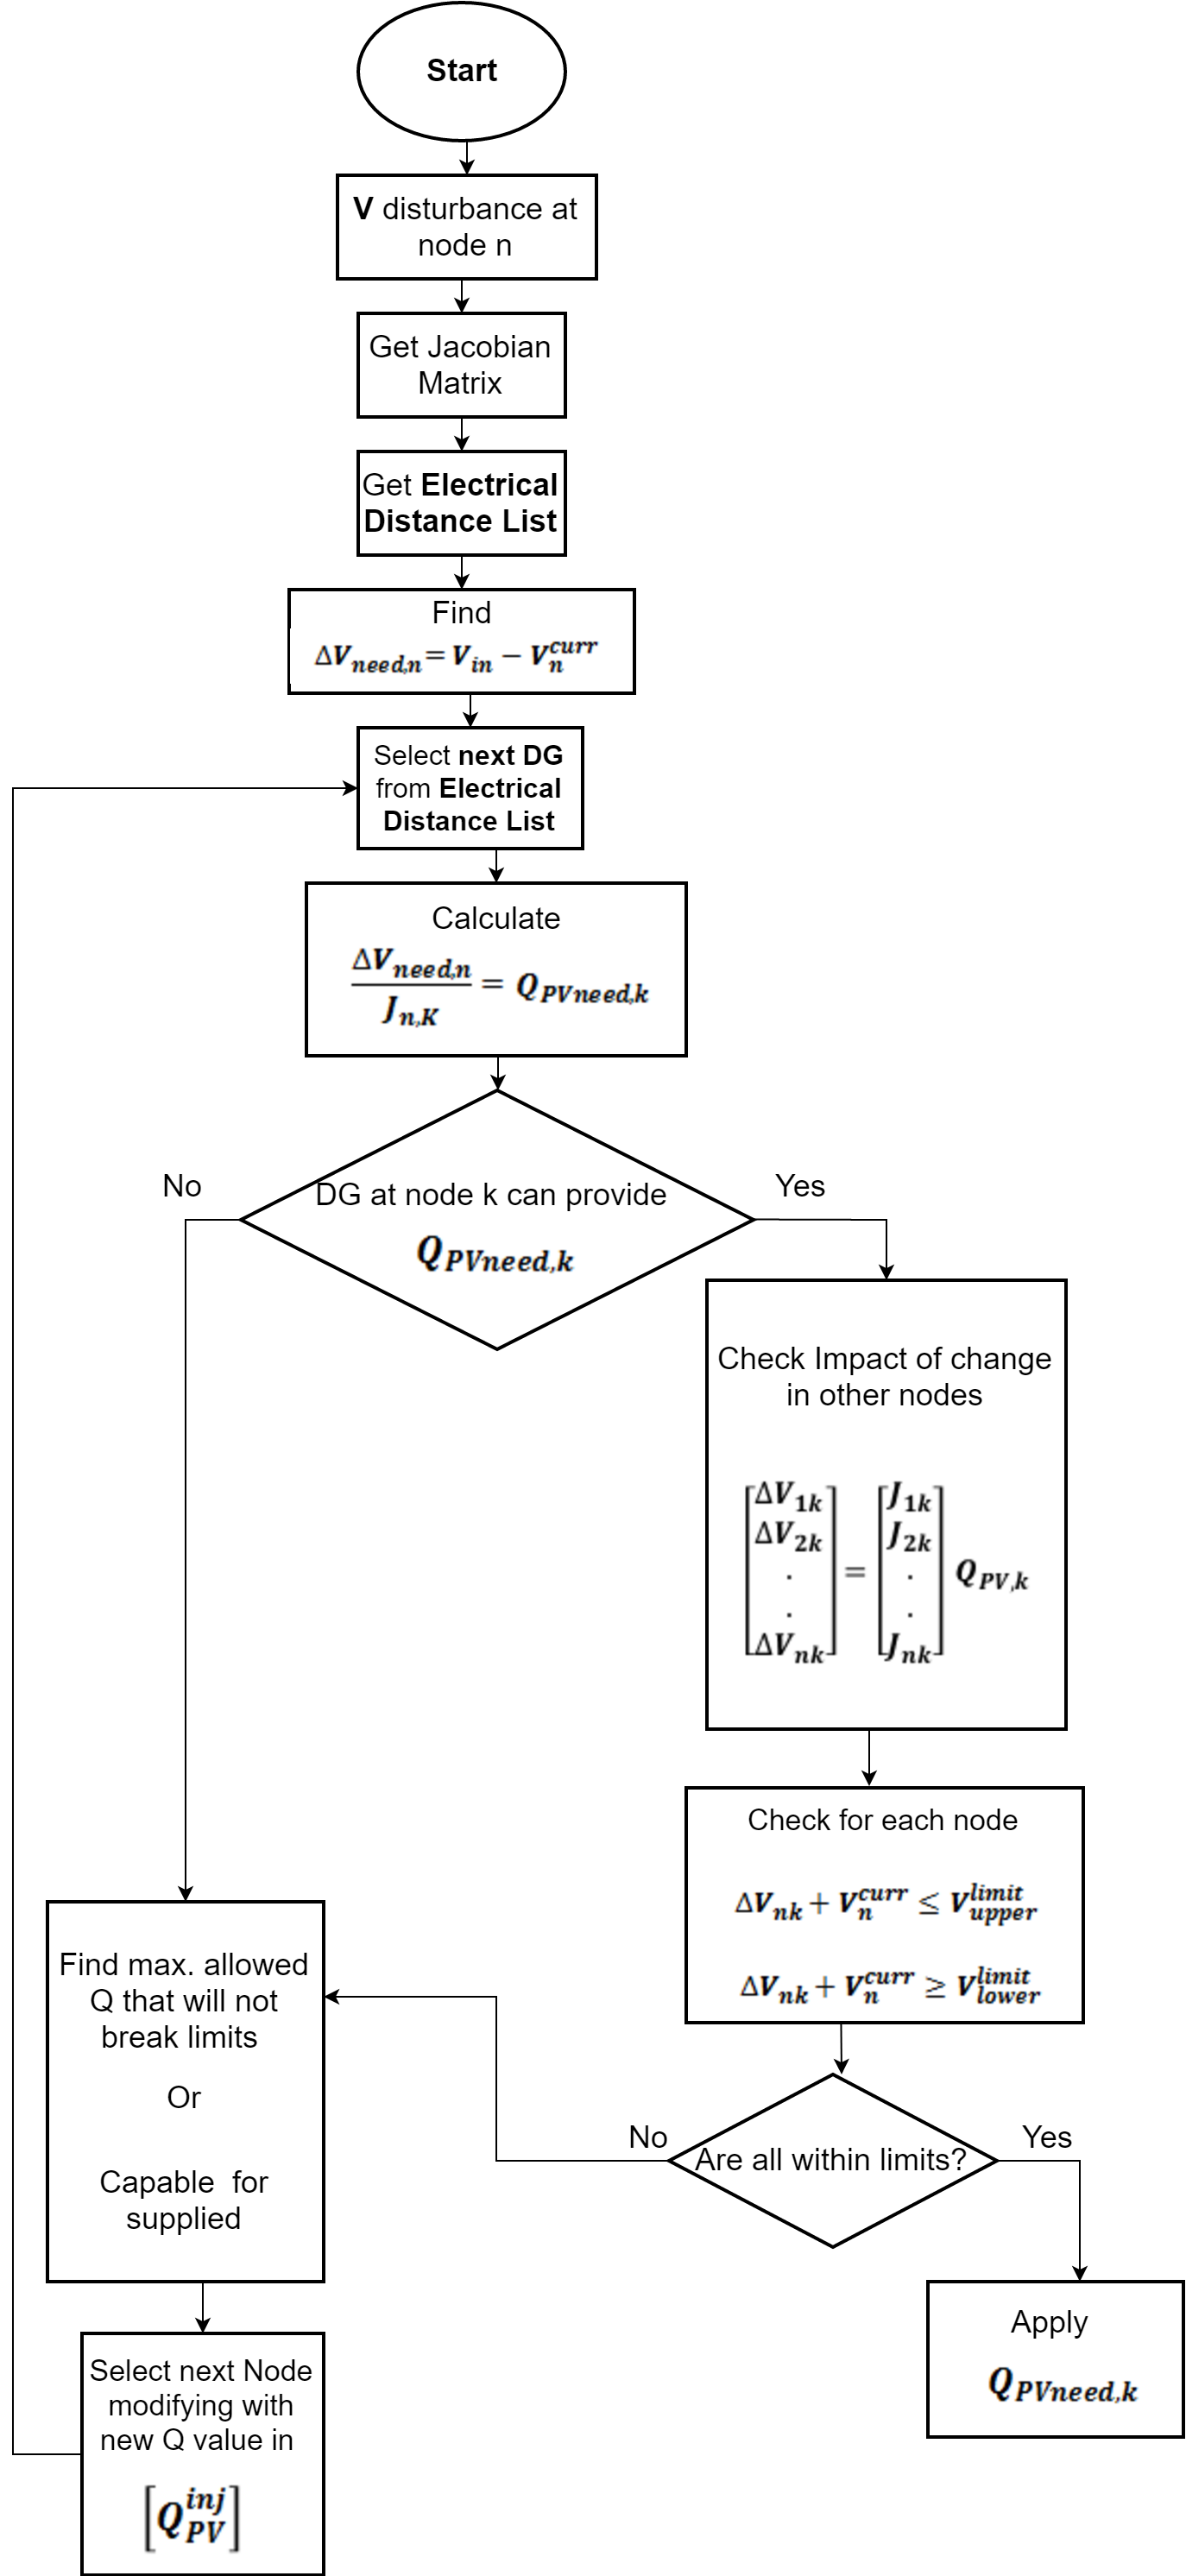
\includegraphics[width=0.5\textwidth]{cvc_alg.png}
% \caption{Coordinated Voltage Control Algorithm Flowchart}
% \label{fig:f1}
% \end{figure}
% The algorithm starts by receiving the needed information from the remote locations. It obtains the voltage and current measurements for each bus and the real and reactive power being generated or absorbed by the DGs. Based on these values, all the voltages are checked against the maximum and minimum voltage range criteria to detect under-voltage or over-voltage issues on specific nodes. When a voltage deviation is detected, the algorithm will start solving the issue from the furthest node to the closest one. The first step in solving this deviation is the application of voltage sensitivity concept to the affected node in order to find the approximate amount of reactive needed be injected at all nodes on control zone of the system. The voltage sensitivity process will return the Jacobian matrix for the system, Jvpq, and the reactive power that each node, in the control zone of the affected bus, needs to individually inject to solve the voltage deviation problem.  After this calculation is completed, a priority list of the nodes on control zone is created based on the criteria of the electrical distances calculated using the method mentioned above. The node closest to the affected node is selected and checked against the nodes that can inject reactive power into the system, in other words, the list of the nodes with DG connected to them. If the node selected to help in the voltage control has the capability of injecting reactive power, the value is checked against all other nodes to assure the compatibility of the value and make sure that no other voltage nodes get out of the desired bounds. As seen on the flowchart, if this value complies with the requirements mentioned, the reactive power reference value is sent to the respective DG inverter. If the value does not comply with the requirements, the next node in the electrical list is selected and the entire process is performed again. Another option for the solution of the reactive power reference calculation, is the application of the maximum reactive power that the current node can supply and the rerun of the entire algorithm to find the solution for the remaining voltage deviation. The algorithm is designed to handle both of these cases and try to minimize the impact in voltage caused by reactive power being injected or absorbed into the system. 




%\subsection{Test System}



\section{Test system}
The distribution network used for testing the coordinated voltage control algorithm is the test system number 2, available under the SUNGRIN project \cite{SG}. This test system was obtained by reducing the network of a larger feeder and it represents a real system in the state of Florida. Fig. \ref{fig:Feeder2} \cite{SG} depicts the topology of the network. The tests were performed considering a balanced system, making it a 9 bus test system. The data for the loads and the PV profiles were also obtained from the SUNGRIN project for that specific location. Fig. \ref{fig:pv_data} shows the real power generation of the three PVs present in the system. The used profile data has a resolution of one minute. Table \ref{tab:load_data} represents the rated values of the loads in the system. Table \ref{tab:Inv_rate} presents the rating of the inverters connected to the PV systems. The inverter reactive power limits (Q limits) are determined by considering a maximum of 0.8 power factor at the point of common coupling. 

\begin{figure}[!h]
\centering
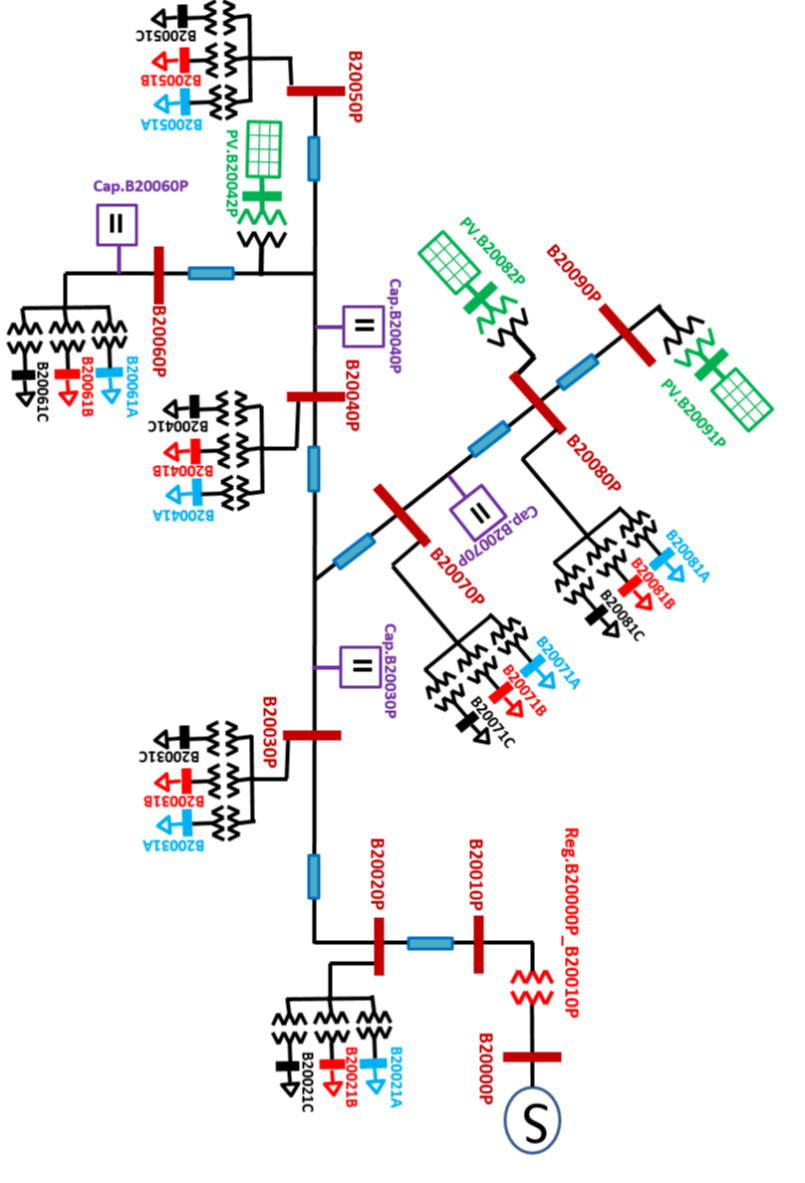
\includegraphics[width=0.85\linewidth]{figs/CVC/feeder_r.png}
\caption{Test Feeder Topology.}
\label{fig:Feeder2}
\end{figure}

\begin{figure}[!h]
\centering
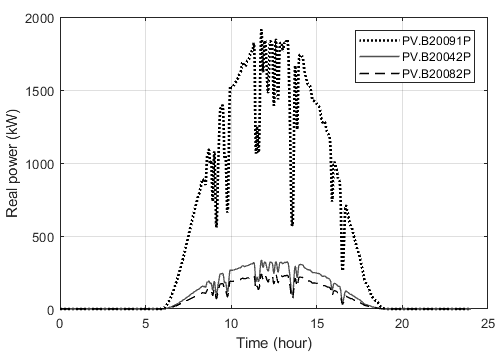
\includegraphics[width=\linewidth]{figs/CVC/PV_DATA.png}
\caption{Test Feeder Topology}
\label{fig:pv_data}
\end{figure}
% \begin{figure}[!h]
% \centering
% 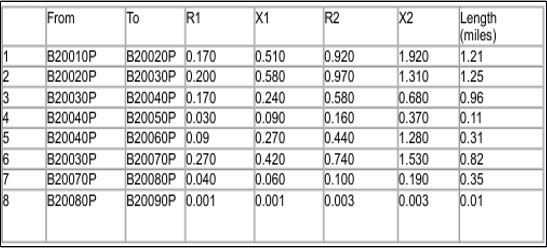
\includegraphics[width=7cm, height=3cm]{linedata.png}
% \caption{Line Data for the Distribution Network}
% \label{fig:BD1}
% \end{figure}

\begin{table}[!h]
\caption{Average load at nodes}
\label{tab:load_data}
\centering
\begin{tabular}{|c|c|c|}
\hline
Load & kVA & Power factor \\ \hline
B20020P & 1035 & 0.90 \\ \hline
B20030P & 2300 & 0.90 \\ \hline
B20040P & 1195 & 0.85 \\ \hline
B20050P & 225 & 0.85 \\ \hline
B20060P & 1285 & 0.85 \\ \hline
B20070P & 1365 & 0.85 \\ \hline
B20080P & 435 & 0.85 \\ \hline
\end{tabular}
\end{table}

% \begin{figure}[!h]
% \centering
% 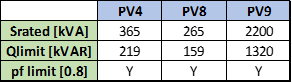
\includegraphics[width=6cm, height=2cm]{pvdata.png}
% \caption{PV Inverter Ratings}
% \label{fig:Inv_rate}
% \end{figure}

\begin{table}[!h]
\centering
\caption{PV Inverter Ratings}
\label{tab:Inv_rate}
\begin{tabular}{c|c|c|c|}
\cline{2-4}
 & PV.B20091P & PV.B20042P & PV.B20082P \\ \hline
\multicolumn{1}{|c|}{Rated power (kVA)} & 365 & 265 & 2200 \\ \hline
\multicolumn{1}{|c|}{Q limit (kVAR)} & 219 & 159 & 1320 \\ \hline
\end{tabular}
\end{table}

\section{Validation and Results}\label{sec:val}
A phasor model of the system shown in Fig. \ref{fig:Feeder2} is modeled and simulated  in MATLAB\textsuperscript{\textregistered} Simulink\textsuperscript{\textregistered} using the Simscape Power Systems\textsuperscript{TM} toolbox for validating the algorithm. Fig. \ref{fig:without_vvc} shows the per-unit feeder bus voltages for 86,400 seconds (24 hours) without implementing the control algorithm. The legends V1, V2, V3, V4, V5, V6, V7, V8 and V9 in the figure represent the per-unit (PU) voltages of buses B20010P, B20020P, B20030P, B20040P, B20050P, B20060P, B20070P, B20080P, and B20090P respectively. As it can be seen in the figure, the bus voltages drop below the 0.95 PU limit when the algorithm is not activated.

\begin{figure}[!h]
\centering
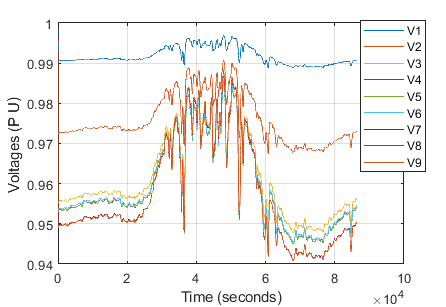
\includegraphics[width=0.6\linewidth]{figs/CVC/Without_VVC.png}
\caption{Voltage Profile without Coordinated Voltage Control}
\label{fig:without_vvc}
\end{figure}

Fig. \ref{fig:with_cvc} presents the voltage profiles of all the nodes in the system with the coordinated voltage control activated. To show the effectiveness of the proposed algorithm the voltage bounds were set between 0.97 PU and 1.01 PU. It can be seen in the figure that the algorithm is capable of maintaining the voltages within the bounds by coordinating the DG inverters and capacitor banks available in the system. Fig. \ref{fig:DG_Q} shows the reactive power supplied by the DGs during the simulation. Fig \ref{fig:cap_bank} shows the switching states of capacitor banks Cap.B20040P, Cap.B20030P and Cap.B20070P. The capacitor bank Cap.B20060P is not used to regulate voltage because it is defined as always on in the system specification. The switching status 1 means that the capacitor bank is connected and the switching status 0 means that the capacitor bank is disconnected. It can be seen from the figures that the coordinated voltage control algorithm was able to maintain the system voltage status within the bounds mostly by using the DG inverters. It required two switching operations from the cap bank Cap.B20070P in addition to the DG inverters capability to maintain system voltage within 0.97 PU and 1.01 PU. It should be noted that during the full 24-hour simulation the on load tap changing transformer situated between buses B20010P and 20000P was not required to control the system voltage. From Fig. \ref{fig:with_cvc} it can also be inferred that the algorithm responds rapidly to voltage violations. In the actual simulation, the algorithm always performed the required calculations under a second.

\begin{figure}[!h]
\centering
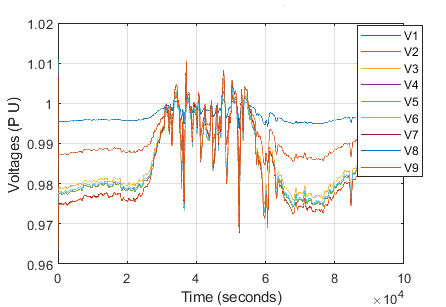
\includegraphics[width=0.6\linewidth]{figs/CVC/With_VVC.png}
\caption{Voltage profile with coordinated voltage control}
\label{fig:with_cvc}
\end{figure}

\begin{figure}[!h]
\centering
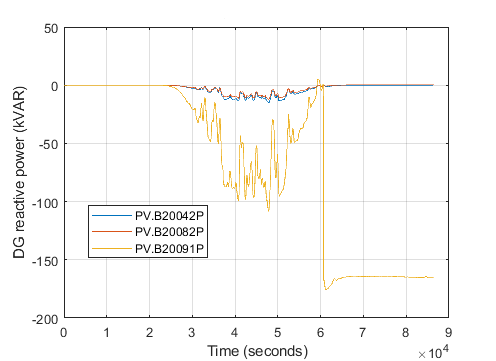
\includegraphics[width=0.6\linewidth]{figs/CVC/DG_Q.png}
\caption{Reactive power supplied by DGs}
\label{fig:DG_Q}
\end{figure}

\begin{figure}[!h]
\centering
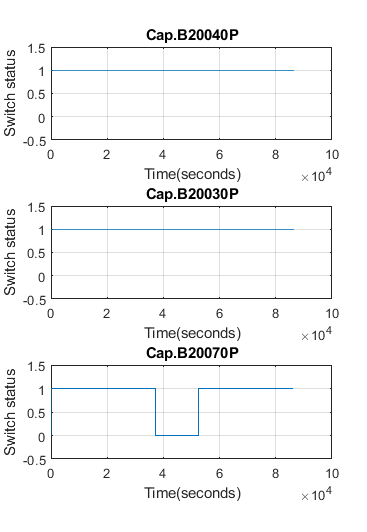
\includegraphics[width=0.5\linewidth]{figs/CVC/CAP_BANK.png}
\caption{Capacitor bank switching states}
\label{fig:cap_bank}
\end{figure}

% \subsection{Offline Validation}
% \subsection{Real-Time validation}

\chapter{Development of Graph Search Based Energy Management for Energy Storage} \label{A8_cahp}
In the last few years, there has been significant growth in grid-connected distributed energy resources (DERs) leading to an increased deployment of distributed generation (DG) and recently more distributed storage (DS) systems. Companies have started to heavily invest in the competitive energy storage system market by taking advantage of the decreasing costs of energy storage. Although a significant amount of DG and DS are being added to the distribution grid, need to improve their control systems for seamless integration to the grid is still there. In the US, most DG and DS systems are deployed to either help reduce the metered load through net-metering programs or to sell power to the utility through power purchase agreements (PPAs). The potential of DG combined with DS is not fully utilized under these pricing schemes due to the lack of proper control schemes. In order to maximize the use of available DERs, a state-of-the-art energy management solution is a necessity for our future smart grid. Such an energy management solution will be able to dynamically optimize the use of all the available DS with the objective of serving the load in the most economical and safe way possible. This will benefit both utility companies and regular consumers. Due to the constraints and intermittent nature of some DG systems, such as wind and solar, the optimum management of DS combined with a DG is a difficult problem to solve. The most common approaches found in the current literature are as follows. Some researchers formulate the problem as a linear programming (LP) or mixed integer linear programming (MILP) model \cite{lp73, lp74, lp75}. Authors in \cite{pso80, pso81} present an energy management solution based on particle swarm optimization for a microgrid containing wind turbines and energy storage (ES) system. Other researchers propose crow-search and ant colony optimization models to solve the energy management problem for local microgrids as seen in \cite{csa87} and \cite{aco84}. There have also been model predictive control (MPC) based approaches for managing ES in microgrid settings as seen in \cite{energymanajaboulay,mpcmorstyn}.  Researchers in \cite{ga76, ga77} have also proposed genetic algorithm based solutions to optimize the ES operation in a microgrid. One clear disadvantage of these proposed models is that most of these approaches only consider the current status of the system and ignore some critical factors like energy tariff, forecasted load, and forecasted generation profiles.  These information can be used to find an optimum solution based on both current and probable future states of the system as opposed to a solution relying only on the currently available data. Off-line day ahead planning models have also been proposed in the literature. In these methods, available predicted data is used to optimize the scheduling of the ES based on Monte Carlo simulations \cite{6872821,7010943,6839110}. These solutions are very computationally intensive and require a lot of time for planning the day ahead. The computational complexity makes them unsuitable for real-time implementation. Also, as they are based on off-line calculations and rely vastly on the accuracy of the predictions.

From the discussion thus far, it is evident that there is a need for a real-time ESM solution that can optimize the long-term operating costs of a system containing DG and an energy storage (ES) system. This paper presents an optimum real-time control strategy for such systems. The proposed control strategy takes into account the present and forecasted states of the system, together with the real-time price (RTP). The rest of the paper is organized as follows.



\section{Problem formulation} \label{formulation}
In this section the problem of optimizing the energy store based on current and forecusted data is formulated. Fig. \ref{fig:system_arch} depicts an example system. Here, the energy storage management system (ESMS) is in charge of controlling the battery connected to the grid with the objective of getting the most cost optimum use of the resources available. The objective of the ESMS is to optimize the use cost of energy storage under different pricing schemes by taking advantage of RTP or time of use (TOU) prices, load and DG generation forecasting.  Fig. \ref{fig:F1_CA} shows the top-level architecture of the ESMS. As seen in the figure, the inputs of the system are the real-time price (RTP) prediction, load prediction, and the DG output prediction, which in this case is a photovoltaic (PV) plant output. It will also consider the current state of the load, current PV generation, and the state of charge of the ES. The output of the ESMS is the optimum battery charge and discharge control references based on the current and forecasted data.

\begin{figure}[!htbp]
\centering
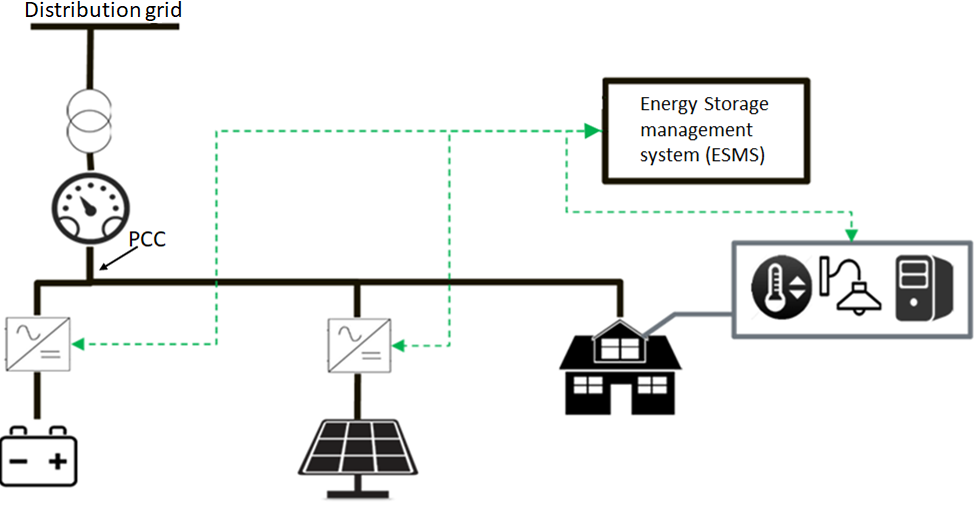
\includegraphics[width=0.6\linewidth]{figs/A8/System_architecture.png}
\caption{Example test system architecture}
\label{fig:system_arch}
\vspace{-3mm}
\end{figure}

%  Fig. \ref{fig:F1_CA} shows the top-level architecture of the ESMS. As seen in the figure, the inputs of the system are the real-time price (RTP) prediction, load prediction, and the DG prediction, which in this case is a photovoltaic (PV) plant. It will also consider the current state of the load, PV generation, and ES. The output of the ESMS is the optimum battery charge and discharge control references based on the current and forecasted data.

\begin{figure}[!ht]
    \centering
    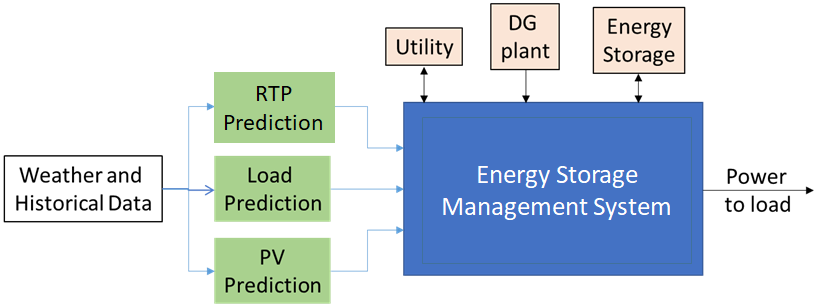
\includegraphics[width = 0.8\linewidth]{figs/A8/EMS_FIG.png}
    \caption{Controller top level architecture}
    \label{fig:F1_CA}
\end{figure}

Determining the optimum reference for the ES in continuous domain is a difficult and computationally intensive tusk. To make the problem solvable is a fast manner the solution space of the problem is discretized. Fig. \ref{fig:F1_Dis} demonstrates an example of the discretized solution space. The horizontal axis of the figure represents time, and the vertical axis represents discrete steps in the state of charge (SOC) of the energy storage. The solution space in the figure assumes that forecast data for the next 45 minutes are available and a control action is taken every 15 minutes. The SOC of the ES is limited between 80\% and 20\%. It is also assumed that the ES can discharge a maximum of 40\% of its maximum SOC and charge a maximum of 20\% of its SOC in a 15 minutes. The space between the upper and lower bounds of the SOC is discretized in steps of 20\%. This allows us to define the solution space as a directional graph. In the graph represented in the figure a discrete value of SOC at a discrete time is a node or a vertex. The possible paths from one node to another node at the next  time step can be defined as a directional edge. Using these definitions the solution space can be defined as a directional graph. The parameters chosen for this simple example are arbitrary. A similar graph can be constructed for various situations based on system properties and constraints.

% In order to find the optimum cost solution based on the current status of the system and future forecasts, the optimization problem is formulated using a graph search problem approach. To represent the solution space of the problem as a graph, the state of charge (SOC) of the ES, and both the prediction horizon and the control horizon are discretized. Fig. \ref{fig:F1_Dis} demonstrates an example of the discretized solution space.
\begin{figure}[!ht]
    \centering
    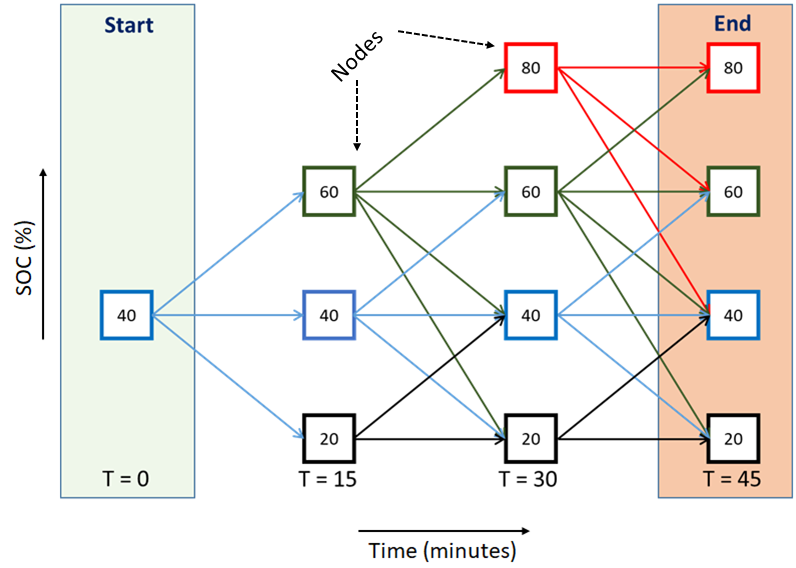
\includegraphics[width = 0.6\linewidth]{figs/A8/F1_1_Dis.png}
    \caption{Discretizing solution space}
    \label{fig:F1_Dis}
\end{figure}

% The horizontal axis of the figure represents time, and the vertical axis represents discrete steps in the state of charge (SOC) of the energy storage. In this simple example scenario, it is assumed that the algorithm recalculates the solution every 15 minutes (control horizon) based on available data. The SOC of the energy storage system (ESS) is discretized in steps of 20\%, and the SOC is limited between 80\% and 20\%. It is also assumed that the ESS can discharge a maximum of 40\% of its maximum SOC and charge a maximum of 20\% of its SOC in a 15 minute time step. These values are chosen arbitrarily in this simple example scenario to explain the problem. Taking these features into consideration, a directed graph is constructed looking ahead three-time steps into the future. The square boxes represent nodes on the graph. The numbers inside the boxes represent the SOC of the ESS at that node. The arrows from the boxes represent all the possible states the ESS can be in the next time step according to the constraints of the system. The arrows are treated as edges of the graph. In this case, the edges are unidirectional. The goal is to find the most cost-efficient path to reach T = 45 minutes. Although in this example the algorithm considers T = 45 as the final stage, in actual application the final stage can be determined based on the actual use case.

\section{A* based energy management system} \label{A*}

\subsection{A* Search Algorithm}
A* is a computer algorithm which is widely used to solve graph search problems \cite{a8book}. It determines the most efficient path between multiple nodes in a graph. A* is an informed search algorithm. This means, it searches between all the possible paths to the goal and finds the path incurring the least cost. To do this, it considers the paths which appear to have the least cost to get to the goal first. Starting from a specific node, it explores the graph step by step depending on the cost of going from one node to the next. The algorithm selects the node to explore based on a combination of the actual cost to get to the node and a heuristic cost that estimates the cost from the current node to the goal. The process to calculate heuristic cost is problem-specific. For the algorithm to work correctly, the heuristic cost has to be less than or equal to the actual cost of getting to the goal node. In other words, the heuristic cost function should never overestimate the cost of reaching the goal. The algorithm works by calculating the combined actual and heuristic cost for all the neighboring nodes of the starting node and puts them into a priority queue called the \textit{open list}. Then, it selects the node with the least cost and expands that node to get the cost of its neighbors. The expanded node is taken out of the priority queue and put in another list called the \textit{closed list}. The algorithm continues to expand the \textit{open list} always selecting the node with the least cost and adding it to the \textit{closed list}. The algorithm terminates when the goal node is inside the \textit{open list}, and it has the minimum cost in the \textit{open list}. Finally, the algorithm retraces its path through the \textit{closed list} to find the optimum route from start to goal. Pseudo code for the A* algorithm is given below.

\textbf{Algorithm 1:} A* search algorithm

\begin{algorithmic}[1]
\label{al:1}
% \Function{heuristic\_estimate}{$a,b$}
%     \State $hCost := \sum_{n=a}^b D(n)*R_{best}(n) $
%     \State \Return $hCost$
% \EndFunction

% \Function{gCost\_calc}{$p,c$}
%     \State $C_{actual}(pc) := C_{ESS}(pc)+C_{GRID}(t)+C_{best}(p)$
%     \State \Return $C_{actual}(pc)$
% \EndFunction

\Function{A*}{$start, goal$}
\State $Closed\_Set = \{\}$ \Comment{Set of evaluated nodes}
\State $Open\_Set = \{Start\}$ \Comment{Set of already discovered nodes which have not been evaluated. Initially,  the start node is discovered.}
\State $Best\_Parent[Start] = \{ \}$ \Comment{It is the node from which the current node can be most effectively reached. At initialization it is empty because the start node has no parent node.}
\State $F\_cost[Start] = G\_cost[Start] + H\_cost[Start]$ \Comment{$F\_cost$ is the combination of the actual cost of reaching a node from the start node \& the heuristic cost of reaching the goal node from the current node. $G\_cost$ is the actual cost \& $H\_cost$ is the heuristic cost of the current node. the Start node has a $G\_cost$ of $0$.}
\While{$Open\_Set$ is not empty}
    \State $Current\_Node = $ node in $Open\_Set$ with lowest $F\_cost$
    \If{$Current\_Node$ == goal}
      \State  \textbf{break} 
    \EndIf
    \For {Each child node of $Current\_Node$}
        \If{Child node in $Closed\_Set$}
            \State \textbf{continue}
        \EndIf
        \If{Child node in $Open\_Set$}
            \If{$G\_cost[child]$ $\geq$ $G\_cost$ already in $Open\_Set$}
                \State \textbf{continue}
            \EndIf
        \EndIf
        \State $Best\_Parent[child] = Current\_Node$
        \State $F\_cost[child] = G\_cost[child] + H\_cost[child]$
        \State $Open\_Set.add(child)$ \Comment{Add child node to $Open\_Set$}

    \EndFor
    \State $Closed\_Set.add(Current\_Node)$ \Comment{Add $Current\_Node$ to $Closed\_Set$}
    \State $Open\_Set.remove(Current\_Node)$ \Comment{Remove $Current\_Node$ From $Open\_Set$}
\EndWhile
\State $Best\_Path = \{ \}$ \Comment{$Best\_Path$ is the most efficient path to get to the goal node.}
\While{$Best\_Parent[Current\_Node] != \{ \}$}
    $Current\_Node = Best\_Parent[Current\_Node]$
    $Best\_Path.add(Current\_Node)$ \Comment{Add $Current\_Node$ to $Best\_Path$}
\EndWhile
\State \Return $Best\_Path$
\EndFunction
\end{algorithmic}

The steps of the algorithm and how it works is explained with a simple example in Fig. \ref{fig:A_STAR_EXAMPLE}. The nodes with white background are the unexplored nodes. The Nodes with orange background are the nodes in open list and nodes with gray background are the nodes in the closed list. The black arrows shows the edges of the graph and the numbers on them represents the cost of taking the edge. The dotted red lines represent heuristic costs from a node to the goal node and their values are represented by the red numbers. The graph shown in the figure is represented as
\begin{equation}
    Z = ( V(Z), X(Z) )
\end{equation}
Here, $V$ is the set of nodes or vertices and $X$ is the set of ordered pairs or edges used the represent the graph Z. Their elements are shown in (\ref{eq:V_Z}) and (\ref{eq:X_Z}) respectively.
\begin{equation}
\label{eq:V_Z}
    V(Z) = \{A,B,C,E,F,G,H\}
\end{equation}
\begin{equation}
\label{eq:X_Z}
    X(Z) = \{ (A,B), (B,E), (E,H), (A,C), (C,G), (C,F), (F,H) \}
\end{equation}

The goal here is to start at node A of Z and find the shorted path to reach node H. In the beginning, Algorithm 1 is given the start node A and goal node H. Then at line 2 the algorithm initializes an empty $Closed\_Set$. Then it initializes the $Open\_Set$ with the starting node which is A in line 3. Then the $F\_cost$ of node A is set to $\infty$ at line 4. These steps are represented in Fig.\ref{fig:A_STAR_EXAMPLE}(a).  Then we enter the while loop in line 5 of the algorithm. As the open set contains the node A the loop continues. On line 6 $Current\_node$ is set to A as A is the only node in open set. Now as $Current\_node$ is not H (goal node) we continue to line 10 of the algorithm. Here, for each child node of $Current\_node$ the algorithm first checks if the node is in closed set. If the child node is in $Closed\_set$ the child node is ignored. Then on lines 14 \& 15 the algorithm checks if the child node is in $Open\_set$ and is the $G\_cost$ of getting to the child is higher than the $G\_cost$ currently present in $Open\_Set$ then the child is ignored. Otherwise we continue with the algorithm and in line 19 the $Current\_Node$ is set as the best parent of the child node. Then the $F\_cost$ of the child node is calculated by adding the $G\_cost$ and $H\_cost$ of the child in line 20. Then the child is added to the $Open\_set$ in line 21. After that in line 23 and 24 of the algorithm the current node is added to the $Closed\_Set$ and taken out of the $Open\_Set$. In the example shown in Fig. \ref{fig:A_STAR_EXAMPLE}, the two children B \& C of node A are explored in this step. As none of them are in $Open\_Set$ or $Closed\_Set$ we calculate the their F costs and add them to the $Open\_Set$. Also node A is taken out of the $Open\_Set$ and added to the $Closed\_Set$. These changes can be noticed in Fig. \ref{fig:A_STAR_EXAMPLE}(b). The gray background behind node A represents that it is in the closed set and the orange backgrounds behind nodes B and C represents they are in the $Open\_Set$. Now the algorithm goes back to line 5 and as $Open\_Set$ is not empty it continues on. This time the node with the lowest cost is B so the children of B are explored. Which reveals the new node E which is added to the $Open\_Set$ and B is taken out of the $Open\_Set$ and added to the $Closed\_Set$. This brings us to the state of the search shown in Fig. \ref{fig:A_STAR_EXAMPLE}(c). $Open\_Set$ not empty so the algorithm continues and chooses node E as current node as it has the lowest $F_Cost$ in the $Open\_Set$. This leads to the discovery of node H which is our goal node. H is added to the $Open\_Set$. E is taken E is taken out of the $Open\_Set$ and added to the $Closed\_Set$. These steps are reflected on Fig. \ref{fig:A_STAR_EXAMPLE}(d). Now we have a path to H and H is the node with the smallest F cost in the $Open\_Set$. SO the algorithm exits the while loop on line 8 and continues to line 26. here best path is initialized as and empty set. Then the algorithm traces back the $Best\_Parent$ of the $Current\_node$ in the while loop between lines 27 to 30 in the algorithm until it reaches the start node. And that gives us the $Best\_Path$. This is shown in Fig. \ref{fig:A_STAR_EXAMPLE_2}. In this case the best path from A to H is A, B, E \& H. This path is shown by the nodes highlighted in blues in the figure.

\begin{figure}[!ht]
    \centering
    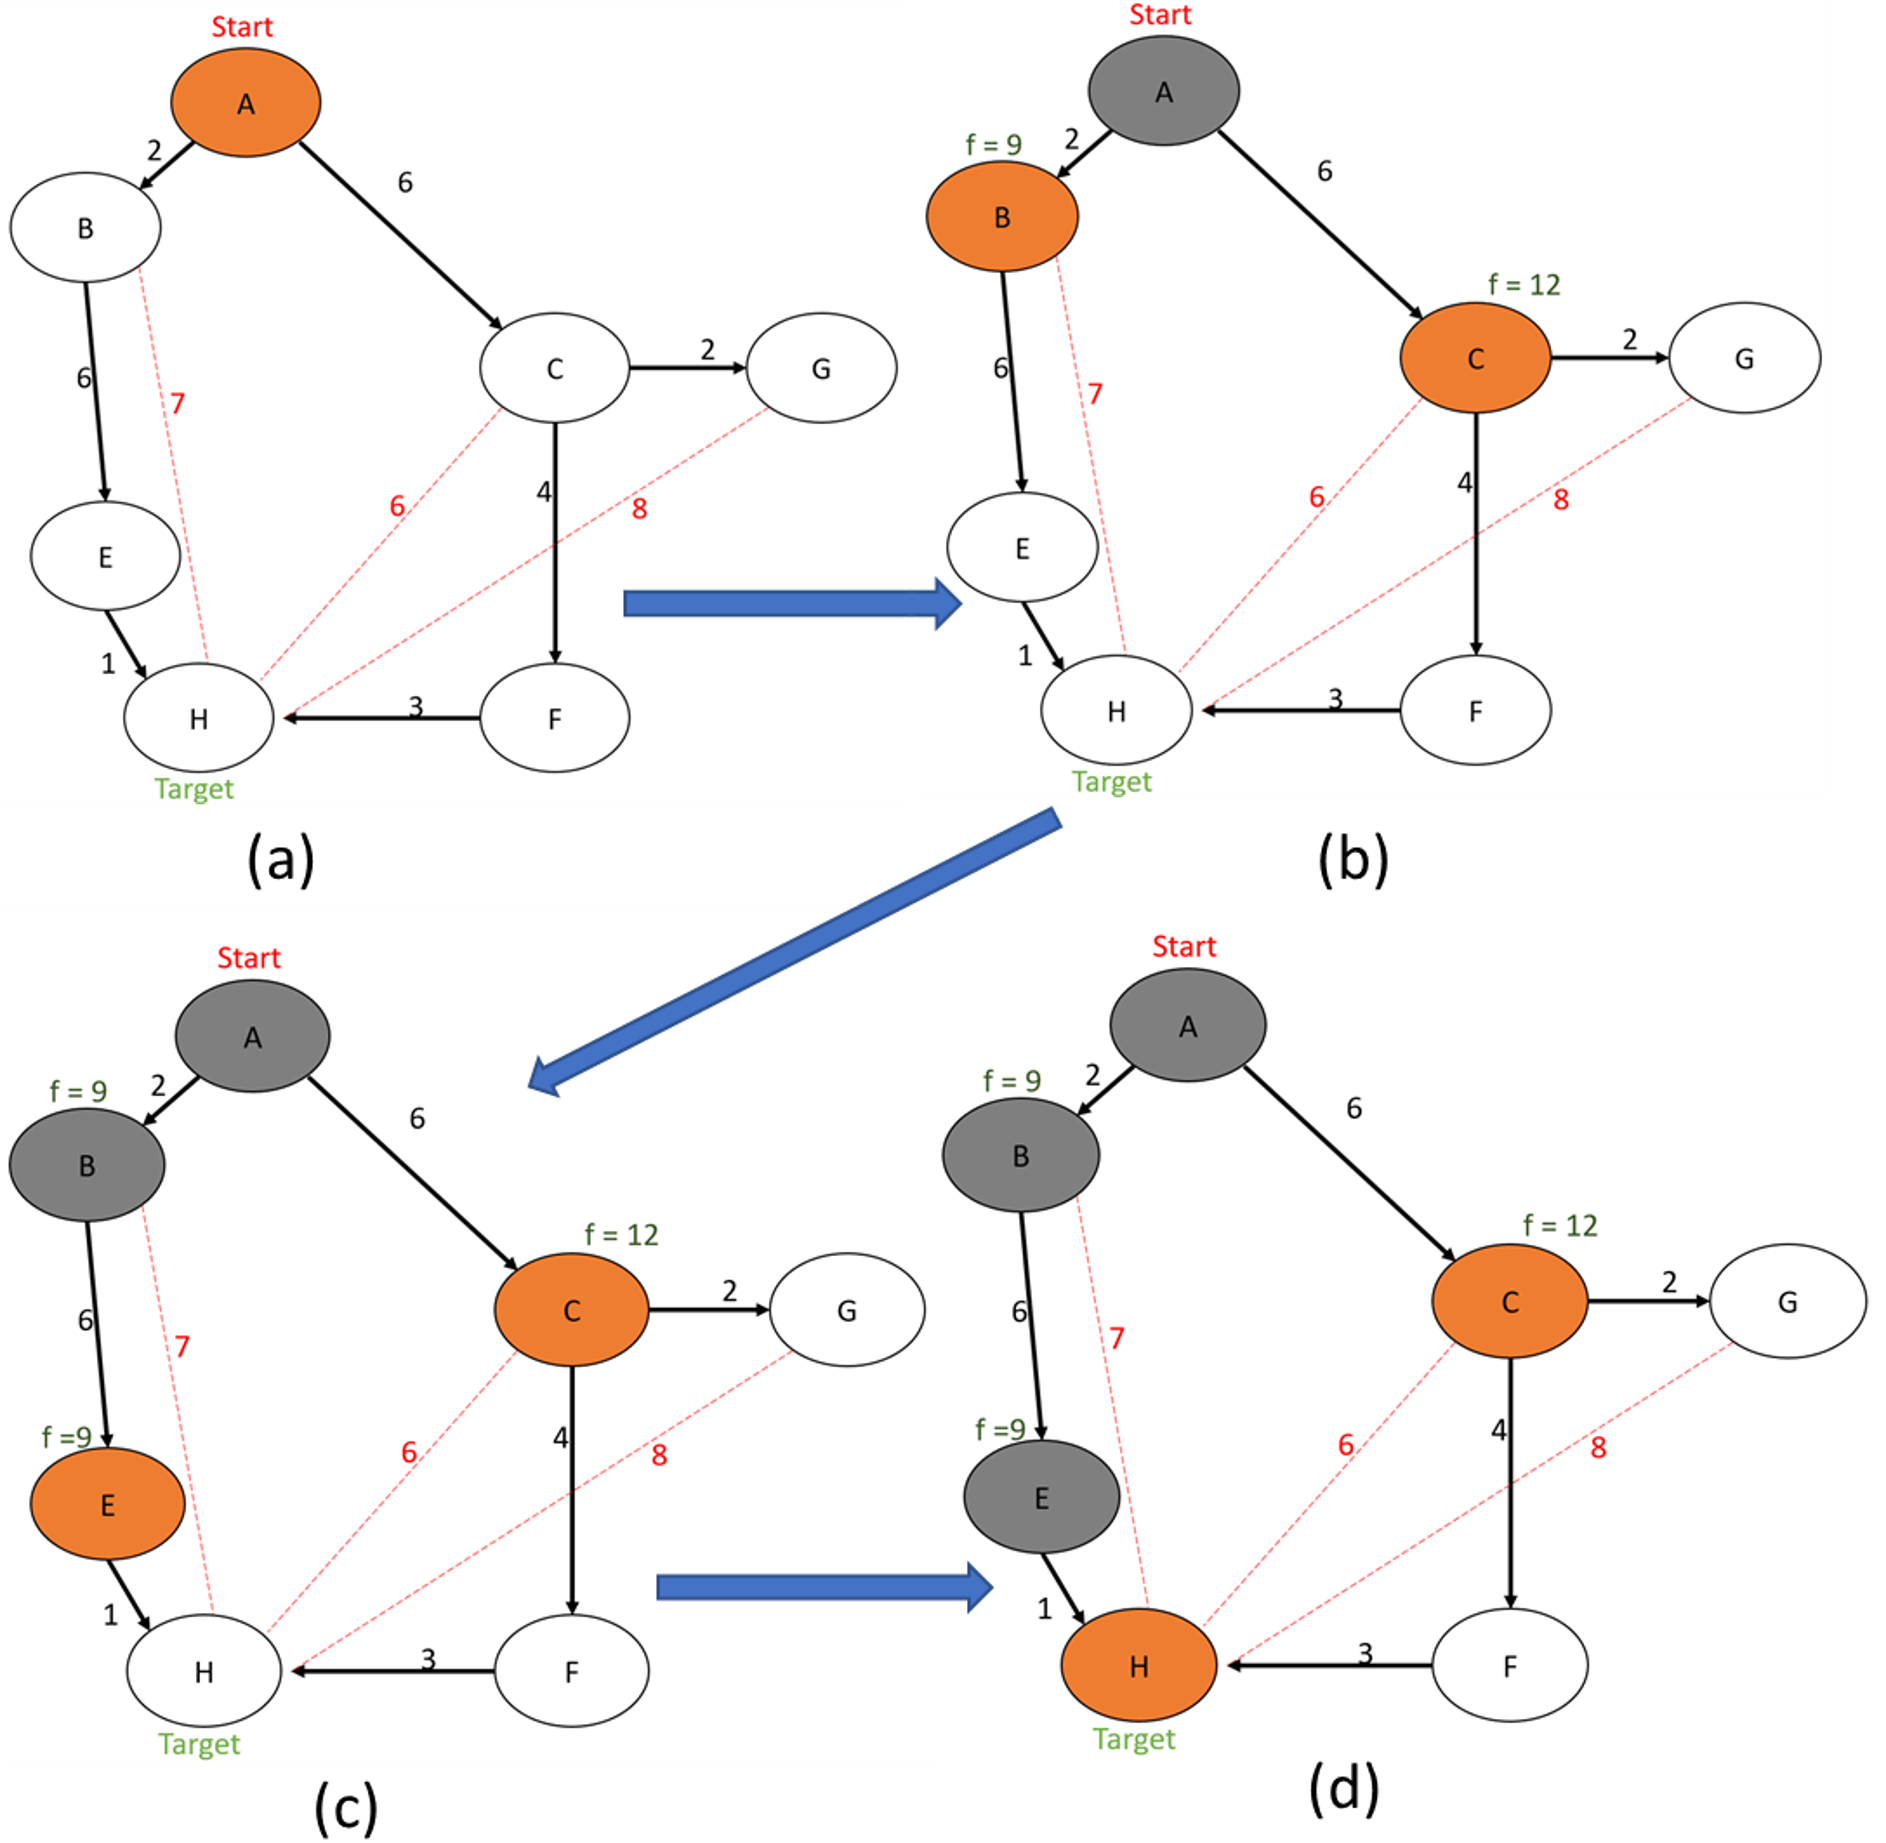
\includegraphics[width = \linewidth]{figs/A8/A_STAR_EXAMPLE.png}
    \caption{A* path finding example to find the shortest path between the nodes A and H of graph Z.}
    \label{fig:A_STAR_EXAMPLE}
\end{figure}


\begin{figure}[!ht]
    \centering
    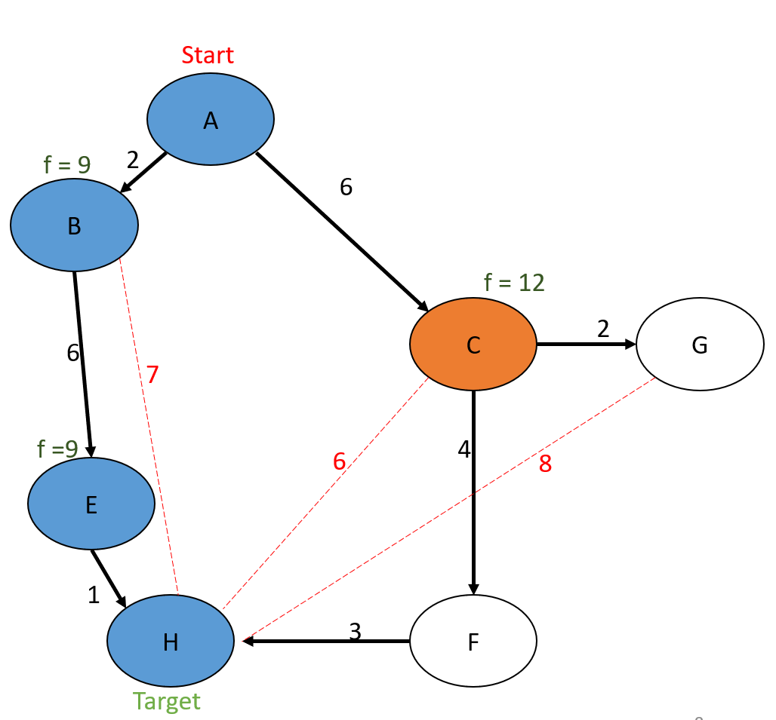
\includegraphics[width = 0.5\linewidth]{figs/A8/A_STAR_EXAMPLE_2.png}
    \caption{A* path finding example best path from A to H.}
    \label{fig:A_STAR_EXAMPLE_2}
\end{figure}


% Fig. \ref{fig:A_STAR_PIC} shows an example of the A* algorithm in a simple directional graph. The capital letters A, B, C, E, F, G and H inside the ellipses represent the nodes of the graph. The starting point of the graph is A, and the goal is to find the shortest path to node H. The solid blue arrows indicate the directional path from one node to the next. The actual cost of taking these paths are represented by the blue numbers beside the solid blue arrows. The red dotted lines represent the heuristic costs from a node to the target (goal) node. The heuristic costs of nodes B, C and G are shown as 7, 6 and 8. The letter 'h' is used to denote this cost. The algorithm starts at node A and discovers the surrounding nodes B and C. The combined heuristic and actual cost of node B is 9 and it is denoted by the letter 'f'. The 'f' cost for node C is 10. So, the algorithm will choose node B as the main candidate to explore. In node B, node E is discovered to have a combined cost of 10. Now, between the nodes C and E, the algorithm will choose a node at random. In this case, let us assume the node selected by the algorithm is E. After expanding E, the algorithm will find a path to node H which costs 10. However, this is still not the lowest path cost among all the nodes in the priority queue. C also has a cost of 10. So, the algorithm will expand the node C and discover two new nodes G and F. The combined heuristic and actual cost of node G is 15 and node F is 14, which in turn are more than 10. So, the algorithm will stop searching and decide that the shortest path from node A to H is the path previously discovered. By using this approach, A* lets us avoid exploring the nodes G and F because the combined heuristic and actual cost of a node are less than or equal to the actual cost taking a path through that node to the target.





% \begin{figure}[!ht]
% \centering
% %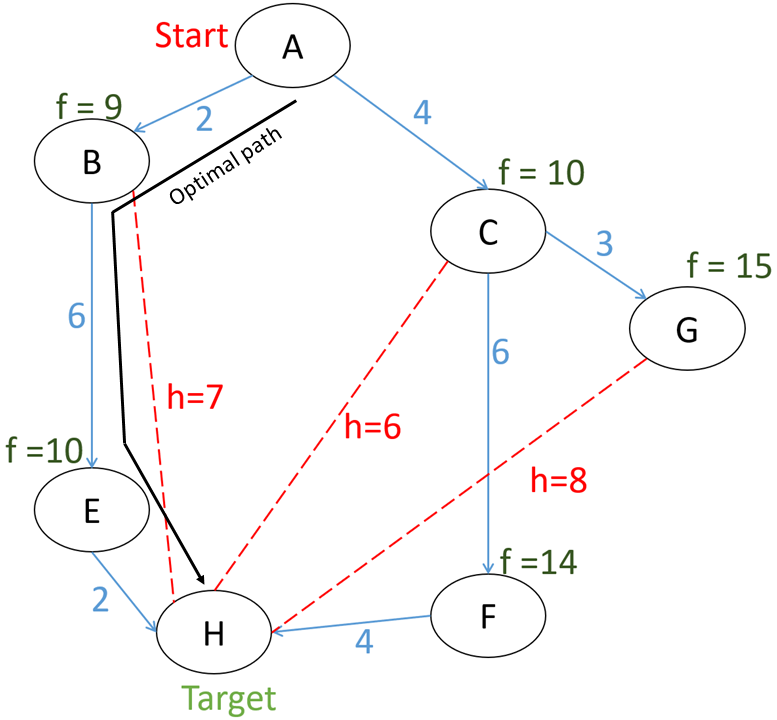
\includegraphics[width=\linewidth]{figs/A_STAR_PIC.png}
% 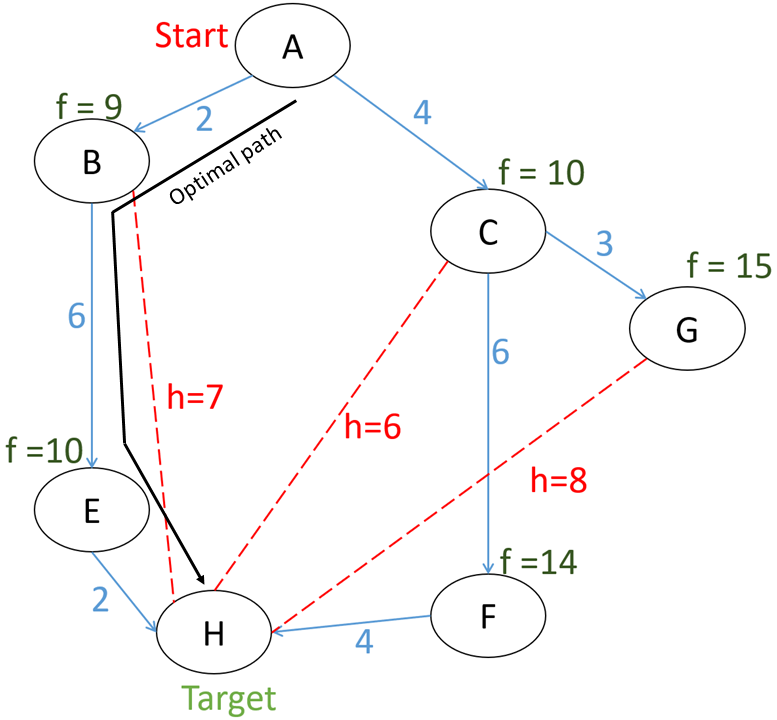
\includegraphics[width=\linewidth]{figs/A_STAR_PIC.png}
% \caption{Example graph for A* implementation}
% \label{fig:A_STAR_PIC}
% \end{figure}

\subsection{Implementation}
By defining the solution space with a combination of nodes and edges, the ESM optimization problem can be formulated as a graph search problem as well. At the inception, the starting node is determined by the current status of the system. Then, the following nodes and edges are generated using the forecasted data available. A discrete set of endpoints are set as the goals of the search. The A* algorithm stops when one of the endpoints are in the $Open\_Set$ and they have the lowest $F\_cost$. The cost of going from a parent node to a child node is calculated by combining the real cost of getting to that child node and the heuristic cost of getting to the goal from that child node. The real cost of going from a parent node $p$ at time $T=t$ to a child node $c$ at time $T=t+\Delta T$ is denoted as $C_{actual}(pc)$. It is calculated according to (\ref{eq:C_actual}).

\begin{equation}
\label{eq:C_actual}
    C_{actual}(pc) =  C_{ESS}(pc)+C_{GRID}(t)+C_{best}(p)
\end{equation}

Here, $\Delta T$ represents the time between two time steps. $C_{actual}(pc)$ represent the total cost of going to the child node $c$ from parent node $p$. $C_{ESS}(pc)$ represent cost of energy storage to go from parent node $p$ to child node $c$. $C_{GRID}(t)$ is the cost of using the grid between time $T=t$ and time $T=t+\Delta T$. $C_{best}(p)$ represent the best or least cost to get to the parent node $p$ from the start node. $C_{ESS}(pc)$ is calculated according to (\ref{eq:C_ESS}).

\begin{equation}
\label{eq:C_ESS}
C_{ESS}(pc) = |(SOC_p - SOC_c)|*ESS_{CAP}*R_{ESS} 
\end{equation}

Here, $SOC_p$ and $SOC_c$ represent the state of charge at parent and child node. $ESS_{CAP}$ represent the total energy capacity of the energy storage. And $R_{ESS}$ is the $\$/kWh$ cost of using the energy storage. $C_{GRID}(t)$ is calculated according to (\ref{eq:C_GRID}).

\begin{equation}
\label{eq:C_GRID}
C_{GRID}(t) = 
\begin{cases}
   E_{GRID}(t)*RTP(t),& \text{if } E_{GRID}(t)\geq 0\\
    E_{GRID}(t)*SP(t),& \text{if }  E_{GRID}(t) < 0
\end{cases}
\end{equation}

Here, $E_{GRID}(t)$ is the energy drawn from the grid between time $T=t$ and time $T=t+\Delta T$. $RTP(t)$ is the real-time price between $t$ and $t+\Delta T$. $SP(t)$ is the price the utility is willing to pay the consumer for selling power between $t$ and $t+\Delta T$. The heuristic cost is calculated by assuming that whichever source has the smallest cost during a time step will supply the total energy demand of that particular time step. The heuristic cost of a node at time $T = t$ is calculated according to (\ref{eq:C_H}).

\begin{equation}
\label{eq:C_H}
C_H(t) = \sum_{n=t}^{end} D(n)*R_{best}(n)
\end{equation}

Here, $C_H(t)$ represents the heuristic cost at time $t$. $D(n)$ is the demand between time $T = n$ and time $T = n+\Delta T$. $R_{best}(n)$ is the source with the smaller cost which is calculated according to (\ref{eq:R_best}).

\begin{equation}
\label{eq:R_best}
R_{best}(n) = 
\begin{cases}
    R_{ESS},& \text{if } RTP(n)\geq R_{ESS}\\
    RTP(n),              & \text{otherwise}
\end{cases}
\end{equation}

After calculating the actual cost  $C_{actual}(pc)$ and heuristic cost $C_H(t)$, the total cost is finally calculated by adding  $C_{actual}(pc)$ and $C_H(t)$.

The EMS recalculates the optimum path using the search algorithm at every time step based on updated information. The system status is assumed to be constant between time steps. 

\section{Test system} \label{sys}
In order to test the proposed A* algorithm, an electric power system (EPS) model based a Florida feeder available in the SUNGRIN report \cite{SUNGRIN} was collected. Fig. \ref{fig:simulation_grid} shows a one-line diagram of the whole system used for testing the algorithm. The dashed borders mark the section of the feeder modified to create a microgrid similar to the one shown in Fig. \ref{fig:system_arch}. The PV and load inside the microgrid are modeled using the load and solar data collected from the SUNGRIN project. An energy storage (ES) system is included to construct the microgrid. Table \ref{tab:solar_pv} shows the physical parameters of the PV plant and its inverter. The energy storage (ES) used in the modeled microgrid has the parameters shown in table \ref{tab:es}. The levelized cost of energy (LCOE)  of the energy storage system $R_{ESS}$ is calculated using (\ref{eq:R_ESS}).

\begin{figure}[!ht]
    \centering
    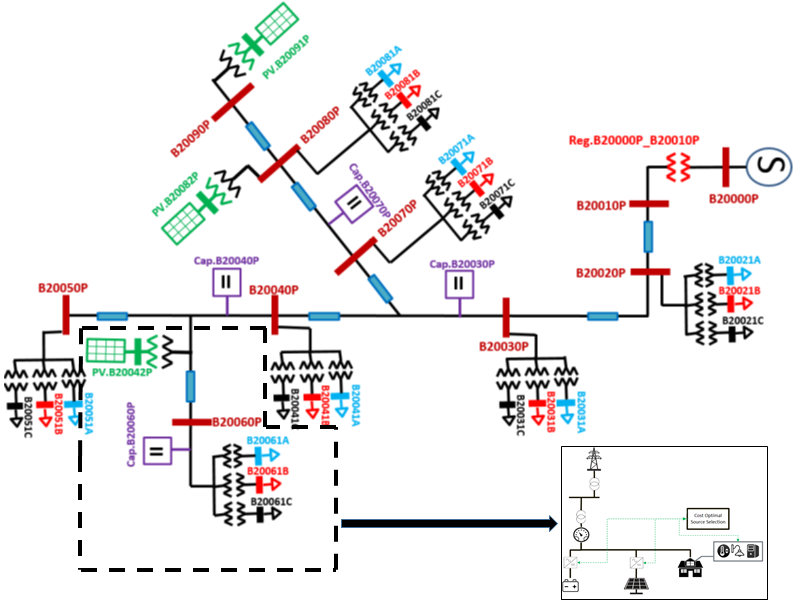
\includegraphics[width = \linewidth]{figs/A8/simulation_grid.png}
    \caption{Simulated system}
    \label{fig:simulation_grid}
\end{figure}


\begin{equation}
\label{eq:R_ESS}
R_{ESS} = \dfrac{ES_{tot}}{Cyc\cdot ES_{Cap}\cdot DoD\cdot \eta_{r}},
\end{equation}

where $ES_{tot}$ is the total cost of the ES system, $DoD$ is the desired depth-of-discharge of the ES system, $Cyc$ is the total number of cycles under warranty at depth-of-discharge, $ES_{Cap}$ is the total energy capacity of the ES system, and $\eta_r$ is the round-trip efficiency of the system. The data used to calculate the $R_{ESS}$ price used in the study were obtained from publicly available data on a commercial ES solution \cite{tesla_powerpack_2018}. 

%%%%%%%%PV%%%%%%%%%%%%%%%%%%%%%%%%%%%%%%%%%%%
\begin{table}[!ht]
%\normalsize
%\renewcommand{\arraystretch}{1}
\caption{PV System Specifications}
\label{tab:solar_pv}
\centering
    \begin{tabular}{ | l | p{3cm} | }
    \hline
    \textbf{PV System Parameters} & \textbf{Value} \\ \hline
    PV Panels Rating (\(P_{PV}\)) & 875 kW  \\ \hline
    Inverter Rating (\(S_{PV}\)) & 900 kVA \\ \hline
    Power Factor Range (\(pf_{PV}\)) & 0.8-1.0  \\ \hline
    Max. Reactive Power (\(\overline{Q_{PV}}\)) & 540 kVAR \\ \hline
    Min. Reactive Power (\(\underline{Q_{PV}}\)) & -540 kVAR \\ \hline
    LCOE (\(r_{PV}\)) & 2.51 c/kWh \\ \hline
    \end{tabular}
    \begin{tabular}{l}
    \end{tabular}
\end{table}
%%%%%%%%PV%%%%%%%%%%%%%%%%%%%%%%%%%%%%%%%%%%%


%%%%%%%%ES%%%%%%%%%%%%%%%%%%%%%%%%%%%%%%%%%%%
\begin{table}[!ht]
%\normalsize
%\renewcommand{\arraystretch}{1}
\caption{Energy Storage (ES) System Specifications}
\label{tab:es}
\centering
    \begin{tabular}{ | l | p{3cm} | p{3cm} | }
    \hline
    \textbf{ES System Parameters} & \textbf{Value} \\ \hline
    ES Rating (\(P_{ES}\)) & 750 kW  \\ \hline
    Inverter Rating (\(S_{ES}\)) & 750 kVA \\ \hline
    Max. State of Charge  (\(\overline{SOC_{ES}}\)) & 2190 kWh \\ \hline
    Min. State of Charge  (\(\underline{SOC_{ES}}\)) & 219 kWh \\ \hline
    Power Factor Range (\(pf_{ES}\)) & 0.8-1.0  \\ \hline
    Max. Reactive Power (\(\overline{Q_{ES}}\)) & 450 kVAR \\ \hline
    Min. Reactive Power (\(\underline{Q_{ES}}\)) & -450 kVAR \\ \hline
    LCOE (\(r_{ES}\)) & 12.3 c/kWh \\ \hline
    \end{tabular}
\end{table}
%%%%%%%%ES%%%%%%%%%%%%%%%%%%%%%%%%%%%%%%%%%%%

Fig. \ref{fig:LOAD_PROFILE_8} shows the load profile of the system for eight days with average, minimum, and maximum load values. To generate the RTP profile, Locational Based Marginal Pricing (LBMP) data were collected from the New York Independent System Operator (NYISO) \cite{NYISO2017}. The collected LBMPO was combined with the time of use (ToU) prices available at Tallahassee to generate an RTP for the proposed test cases. Another price profile was collected from the PG\&E peak day pricing scheme \cite{pgne}. Both profiles were used as RTP profiles to validate the algorithm under different pricing schemes. Fig. \ref{fig:RTP_PROFILE_8} shows the real-time price (RTP) profiles used for testing the proposed system. The solid lines represent the price profile collected from NYISO and the dashed lines represent the price profile collected from PG\&E. The eight-day PV and load profile used for the test system was collected from the SUNGRIN project and scaled to fit the ratings of the PV described in Table \ref{tab:solar_pv}. Fig. \ref{fig:PV_PROFILE_8} shows the eight-day PV profile used.

\begin{figure}[!ht]
    \centering
    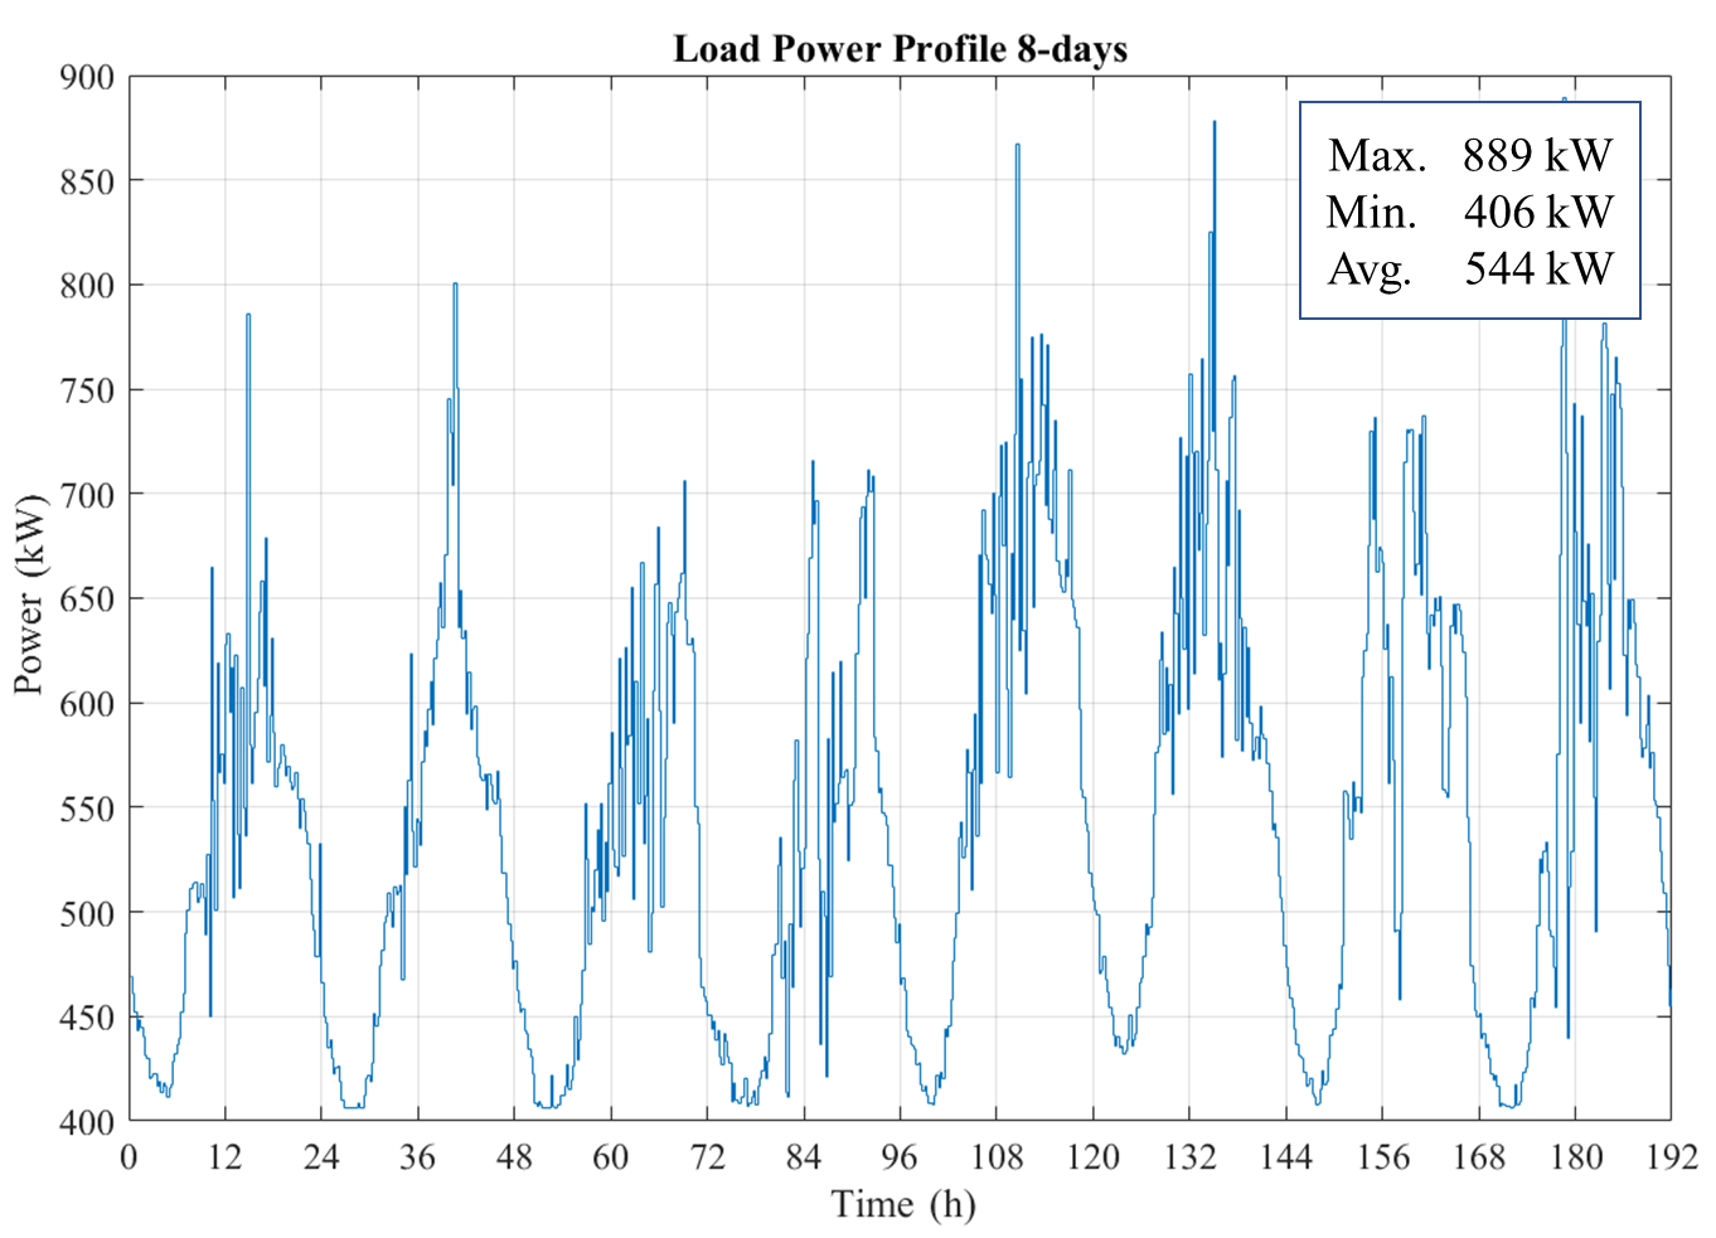
\includegraphics[width = \linewidth]{figs/A8/loadprofile.png}
    \caption{Eight day load profile}
    \label{fig:LOAD_PROFILE_8}
\end{figure}

\begin{figure}[!ht]
    \centering
    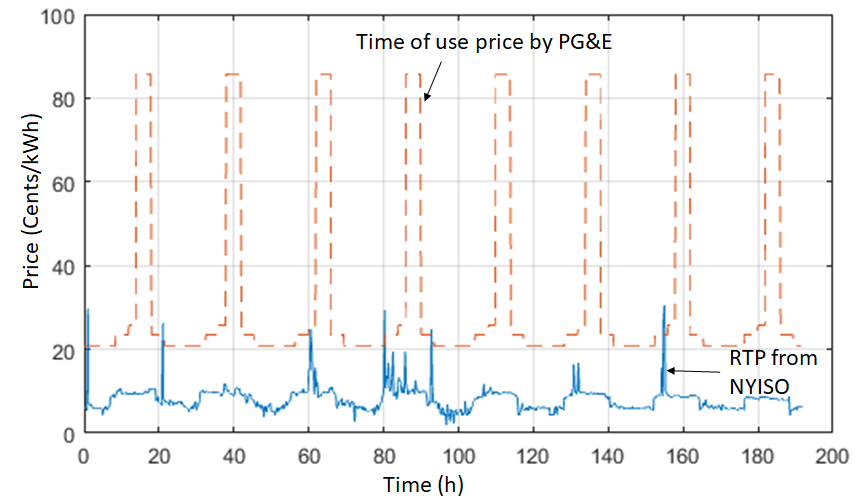
\includegraphics[width = \linewidth]{figs/A8/Price_profiles.png}
    \caption{Eight day RTP profile NYISO}
    \label{fig:RTP_PROFILE_8}
\end{figure}

% \begin{figure}[!ht]
%     \centering
%     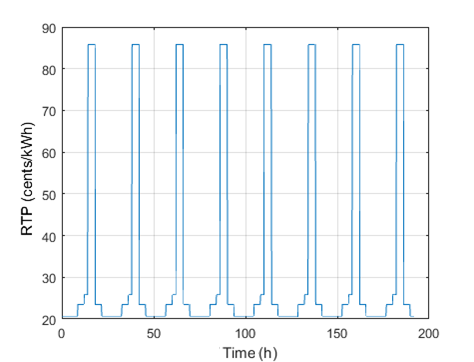
\includegraphics[width = \linewidth]{figs/PGNE_PRICE.png}
%     \caption{Eight day RTP profile PG\&E}
%     \label{fig:PGNE_PRICE}
% \end{figure}


\begin{figure}[!ht]
    \centering
    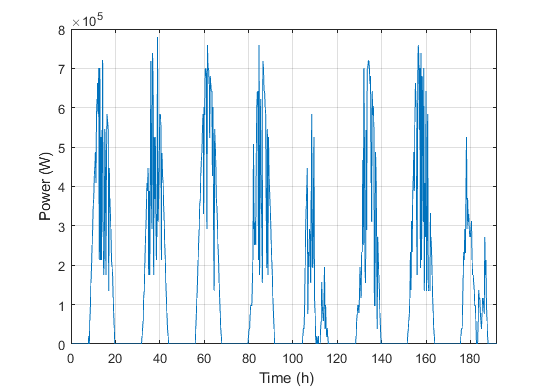
\includegraphics[width = \linewidth]{figs/A8/PV_PROFILE.png}
    \caption{Eight day PV profile}
    \label{fig:PV_PROFILE_8}
\end{figure}




\section{Offline simulation and results} \label{OFF}
The system described in Section \ref{sys} is modeled and simulated in MATLAB\textsuperscript{\textregistered} Simulink\textsuperscript{\textregistered} using the Simscape Power Systems\textsuperscript{TM} toolbox in phasor domain for the Offline simulation. The A* based ESM is run using the described data, and the results are fed in as an open loop control to a Simulink model for phasor simulation. In the test cases, the energy management problem is formulated according to the formulation discussed in Section \ref{formulation}. The  SOC of the ESS is discretized in steps of 2\%, and the SOC is limited between  94\%  and  10\%. The time step and the control horizon chosen is 15 minutes. The ES is allowed to charge or discharge a maximum of 8\% of its total capacity during one time-step. The 8\% limitation is set based on the power specifications discussed in table \ref{tab:es}. The A* search runs every 15 minutes considering a 24 hours (96 time-steps) prediction horizon. The performance of the A* based ESM is compared against two sample base test cases. The base test cases are the following:

\begin{enumerate}
\item \textbf{Case 1:} Charging the ES from 2 AM to 5 AM, Discharging the ES from 7 PM to 11 PM

\item \textbf{Case 2:} Charging from the ES 11 AM to 2 PM, Discharging the ES from 7 PM to 11 PM
\end{enumerate}

All the test cases are run under two different scenarios. The scenario I considers Net Metering Scheme and  Scenarios II considers different prices for buying and selling energy. 

\subsection{Scenario I: Net Metering} \label{netmeter}
In this scenario, the A* based EMS is compared against the two base test cases considering net metering. The NYISO RTP scheme shown in Fig. \ref{fig:RTP_PROFILE_8} is used for this comparison. The price of energy storage is chosen as 12.6 \cent/kWh. This price is calculated based on the specifications of the Tesla Powerpack \cite{tesla_powerpack_2018}.

Fig. \ref{fig:SBMPO_COMP_1_day} shows a zoomed view of the first day of the 7-day simulation for the A* based EMS. The solid black line in the figure represents the SOC of the energy storage, and the dotted red line represents the RTP. The dashed blue line represents the apparent demand. The left vertical axis of the graph represents the RTP of energy and the SOC of the ES. The right vertical axis represents the kWh apparent demand (actual demand - PV generation) of the system. A negative apparent demand represents excess energy from the local generation after fulfilling the local demand. The horizontal axis represents time in hours. The arrows with the numbers are showing specific points of the figure that are explained next, based on the behavior of the EMS. As observed in Fig. \ref{fig:SBMPO_COMP_1_day}, there are two peaks in price at the points 1 and 3 throughout the 24 hours window of operation. The ESM accurately anticipates the price peak in point 1 and charges the energy storage using the grid just before the peak occurs, and discharges during the price peak at point 1. It can be seen that during the peak, the apparent demand was positive and the lowest available price for grid energy was available just before the peak. The algorithm also anticipates the next price peak at point 3 based on forecasted data and prepares the ES to discharge at that price peak by charging at the lowest RTP period at point 2. Although, there is excess generation available from the PV in between point 2 and point 3 the opportunity cost of using the PV to charge the ES will be equal to the RTP due to net metering. So, in this case, the algorithm behaves as expected and uses the lowest possible RTP period to charge the ES and discharges during the price period when there is a high enough price peak to justify the use of the energy storage.

\begin{figure}[!ht]
    \centering
    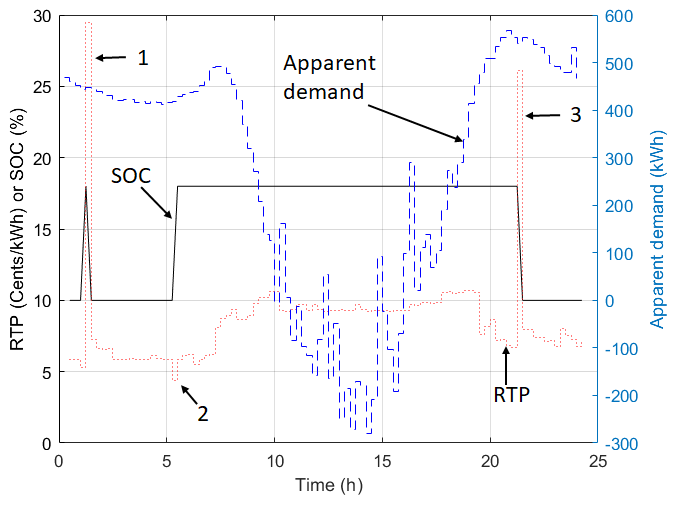
\includegraphics[width = 0.7\linewidth]{figs/A8/SBMPO_COMP_1_day.png}
    \caption{First day EMS response for net metering comparison case}
    \label{fig:SBMPO_COMP_1_day}
\end{figure}

Fig. \ref{fig:SBMPO_COMP_10_12} shows the response of the A*-based EMS in a seven days run used in the same microgrid system.  It can be seen from the figure that the A*-based ESM is following the same behavior displayed in Fig. \ref{fig:SBMPO_COMP_1_day}. It is taking advantage of the lowest energy price before a price peak appears in its prediction horizon, and charging the energy storage in order to discharge it when there is a high enough price peak. The total cost of operation for the A*-based ESM for the seven day period is shown in Table \ref{tab:Cost1}

\begin{table}[htb]
\caption{Seven day Cost for the three cases (net metering)}
\centering
\label{tab:Cost1}
\begin{tabular}{|l|l|}
\hline
Case1 & \$7,086 \\ \hline
Case2 & \$8,601 \\ \hline
A* Case & \$4,861 \\ \hline
A* Case \% savings (Case1) & 31.40\% \\ \hline
A* Case \% savings (Case2) & 43.48\% \\ \hline

\end{tabular}
\end{table}

\begin{figure}[!ht]
    \centering
    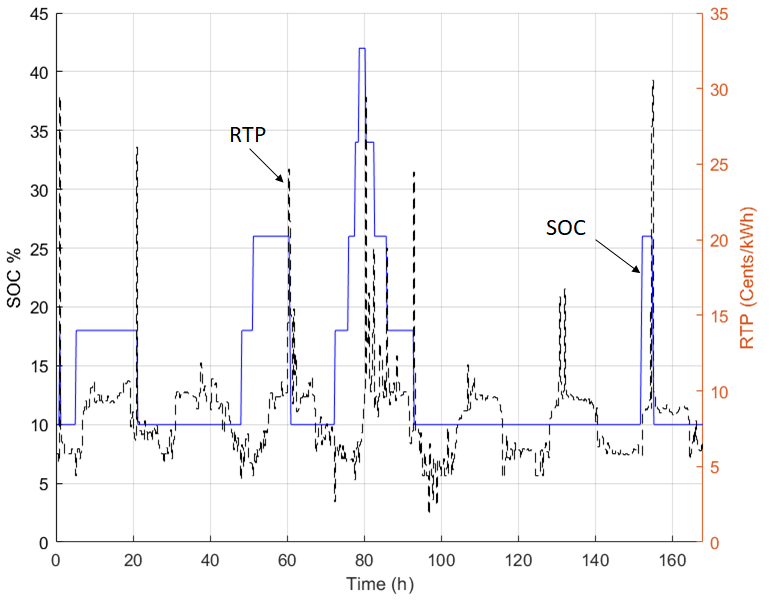
\includegraphics[width = 0.7\linewidth]{figs/A8/SBMPO_COMP_10_12.png}
    \caption{Full 7 day EMS response for net metering comparison case}
    \label{fig:SBMPO_COMP_10_12}
\end{figure}

\subsection{Scenario II: Buying and Selling Prices are Different}
In this scenario, the proposed algorithm is tested against the two base test cases using different price for selling power back to the grid. The cases 1 and 2 are previously fixed standard control strategies based on predefined charging and discharging of the energy storage mentioned before. The only difference is that the buying and selling price of energy from the grid is not the RTP. It is considered that the consumer is only allowed to sell power back to the grid at a rate of 4 cents/kWh.

Fig. \ref{fig:VAR_1_day_example} shows the 1-day test result for the A*-based EMS considering the RTP scheme shown in Fig. \ref{fig:RTP_PROFILE_8} for buying power and considering a sell-back price of 4 cents/kWh. The other system parameters are kept the same as the system used in the previous scenario. As seen in Fig. \ref{fig:VAR_1_day_example}, there are two peaks in price at the points 1 and 3 throughout the 24-hour window of operation. The ESM correctly anticipates the peak at point 1 and charges the energy storage using the grid just before the peak occurs and discharges during the price peak at point 1, similar to the behavior observed in the previous scenario. The next price peak is at point 3, and the lowest price for grid power available for charging the storage is at point 4. In case of a net metering scheme, point 4 would have been the best time to charge the ES in order to discharge it during the next price peak. However, since a sell-back price of 4 cents/kWh is being considered, this is no longer the case. The price 4 cents/kWh is lower than the price of buying grid energy at point 4. So the A*-based EMS takes into account that the opportunity cost for using power during point 2 instead of selling it back to the grid is 4 cents/kWh and decides to charge the ES during point 2 when there is additional local generation available. This behavior demonstrates that the A*-based ESM can use the forecasted knowledge of the future demand and RTP together to automatically decide the best moments to operate the energy storage depending on different pricing schemes.

 \begin{figure}[!ht]
    \centering
    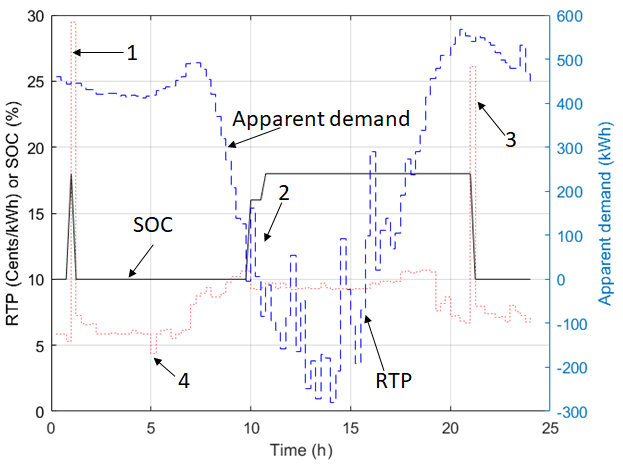
\includegraphics[width = 0.7\linewidth]{figs/A8/VAR_1_day_example.png}
    \caption{1 day EMS response considering NYISO price and 4 centes/kWh sellback price}
    \label{fig:VAR_1_day_example}
\end{figure}

Fig. \ref{fig:VAR_10_12_4} shows the 7-day test result for the tested microgrid considering the RTP shown in Fig. \ref{fig:RTP_PROFILE_8} and a sell-back price of 4 cents/kWh. Fig. \ref{fig:PG_VAR_10_12_4} show the ESM operation for the PG\&E profile shown in Fig. \ref{fig:RTP_PROFILE_8} considering 4 cents/kWh sell-back price. It can be observed from the 7-day cases, that the A*-based ESM shows behavior similar to the behavior seen in  Fig. \ref{fig:VAR_1_day_example}. The ESM scheme was also tested considering a sell-back price of 30\% of RTP for both the NYISO and PG\&E price profiles. The costs for the different conditions considered in the three cases are shown in Table \ref{tab:Cost}. Depending on the test case evaluated, the A* based ESM shows substantial cost savings of around 6.93\% to 41.79\%. 

 \begin{figure}[!ht]
    \centering
    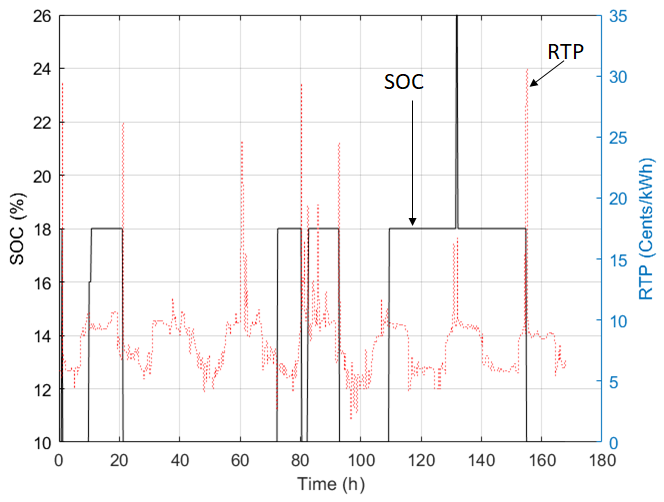
\includegraphics[width = 0.7\linewidth]{figs/A8/VAR_10_12_4.png}
    \caption{7 day EMS response considering NYISO price and 4 centes/kWh sell back price}
    \label{fig:VAR_10_12_4}
\end{figure}

%  \begin{figure}[!ht]
%     \centering
%     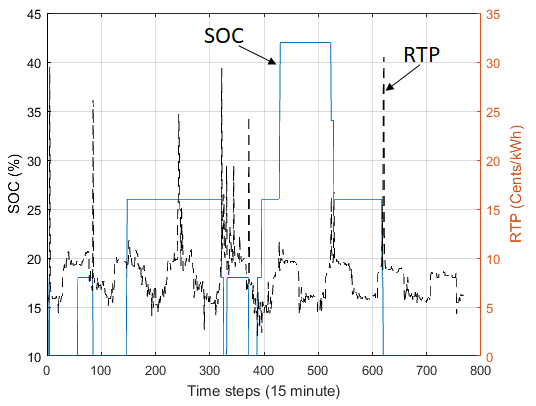
\includegraphics[width = \linewidth]{figs/VAR_10_12_30rtp.png}
%     \caption{7 day EMS response considering NYISO price and 30\% of RTP sell back price}
%     \label{fig:VAR_10_12_30rtp}
% \end{figure}

 \begin{figure}[!ht]
    \centering
    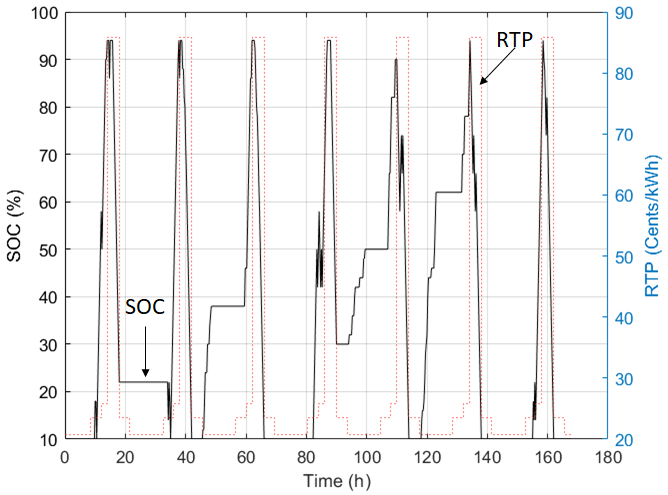
\includegraphics[width = 0.7\linewidth]{figs/A8/PG_VAR_10_12_4.png}
    \caption{7 day EMS response considering PG\&E price and 4 centes/kWh sell back price}
    \label{fig:PG_VAR_10_12_4}
\end{figure}

%  \begin{figure}[!ht]
%     \centering
%     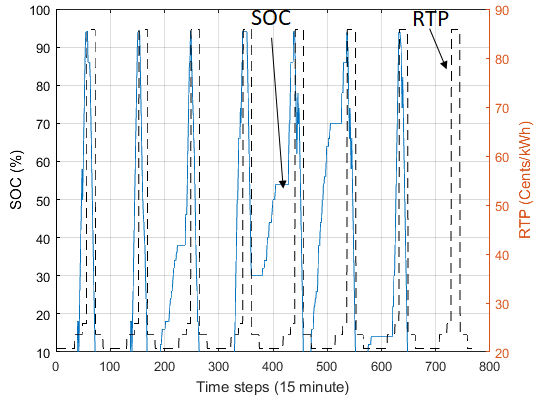
\includegraphics[width = \linewidth]{figs/PG_VAR_10_12_30rtp.png}
%     \caption{7 day EMS response considering PG\&E price and 30\% of RTP sell back price}
%     \label{fig:PG_VAR_10_12_30rtp}
% \end{figure}


%%%%%%%%CSOT%%%%%%%%%%%%%%%%%%%%%%%%%%%%%%%%%%%
\begin{table}[htb]
%\normalsize
%\renewcommand{\arraystretch}{1}
\caption{Seven day Cost for the three cases (different sell price)}
\label{tab:Cost}
\centering

\begin{tabular}{l|l|l|l|l|}
\cline{2-5}
                            & \multicolumn{2}{l|}{4 cents/kWh} & \multicolumn{2}{l|}{30\% RTP}   \\ \cline{2-5} 
                            & NYISO           & PG\&E          & NYISO          & PG\&E          \\ \hline
\multicolumn{1}{|l|}{Case1 cost} & \$8,265  & \$19,396 & \$8,314 & \$19,109 \\ \hline
\multicolumn{1}{|l|}{Case2 cost} & \$8,8606  & \$19,633 & \$8,895 & \$19,407 \\ \hline
\multicolumn{1}{|l|}{A* Case cost} & \$5,329  & \$18,051 & \$5,178 & \$17,106 \\ \hline
\multicolumn{1}{|l|}{A* Case \% savings (Case1)} & 35.52\%         & 6.93\%         & 37.72\%        & 10.84\%        \\ \hline
\multicolumn{1}{|l|}{A* Case \% savings (Case2)} & 39.85\%         & 8.08\%         & 41.79\%        & 11.86\%        \\ \hline
\end{tabular}

\end{table}
%%%%%%%%CSOT%%%%%%%%%%%%%%%%%%%%%%%%%%%%%%%%%%%%%%%%%%%

%%%%%%%%COMPARE_COST%%%%%%%%%%%%%%%%%%%%%%%%%%%%%%%%%%%
% \begin{table}[htb]
% %\normalsize
% %\renewcommand{\arraystretch}{1}
% \caption{Case 3 savings compared to other cases (7 days)}
% \label{tab:Cost_comp}
% \centering
% \begin{tabular}{l|l|l|l|l|}
% \cline{2-5}
%                             & \multicolumn{2}{l|}{4 cents/kWh} & \multicolumn{2}{l|}{30\% RTP}   \\ \cline{2-5} 
%                             & NYISO           & PG\&E          & NYISO          & PG\&E          \\ \hline
% \multicolumn{1}{|l|}{Case1} & 35.52\%         & 6.93\%         & 37.72\%        & 10.84\%        \\ \hline
% \multicolumn{1}{|l|}{Case2} & 39.85\%         & 8.08\%         & 41.79\%        & 11.86\%        \\ \hline
% \end{tabular}
% \end{table}
% %%%%%%%%COMPARE_COST%%%%%%%%%%%%%%%%%%%%%%%%%%%%%%%%%%%

\section{Real-time simulation and results} \label{RT}
A controller hardware in the loop (CHIL) simulation was set up to validate the algorithm in a real-time environment. 
The block layout of the CHIL simulation is shown in Fig. \ref{fig:RT_block}. The power system shown in Fig. \ref{fig:simulation_grid}, is simulated in real time in a digital real-time simulator (DRTS) with a time step of 50 ${\mu}s$. This system is modeled for detailed electromagnetic transient simulation unlike the phasor simulation model used in the offline simulation. The A* based ESM algorithm is implemented in Python 2.7 on a windows machine. The specifications of the machine are given in Table \ref{tab:PC}. The communication link between the DRTS and windows machine was established using TCP/IP. The DRTS sent the windows machine running the ESM the current PV generation ($P_{PV}(t)$), the current load ($P_load(t)$) and the current energy storage state of charge ($ES_{SOC}(t)$). The RTP, Load and PV prediction profiles are fed to the ESM by a pregenerated MATLAB formatted data (MAT) file. The current RTP is also provided by the MAT file. After receiving the current status and predicted profiles the ESM determines the power the ES should provide for the current time period ($P_{ES}(t)$) and sends it back to the DRTS. The actual CHIL setup is shown in Fig. \ref{fig:LAB_REAL}.

\begin{table}[htb]
\caption{Windows machine specification}
\label{tab:PC}
\centering
\begin{tabular}{|l|l|}
\hline
Operating system & Windows 10 Home 64-bit      \\ \hline
Processor        & Intel(R) Core(TM) i5-7300HQ \\ \hline
Memory           & 8192 MB RAM                 \\ \hline
\end{tabular}
\end{table}

\begin{figure}[!ht]
    \centering
    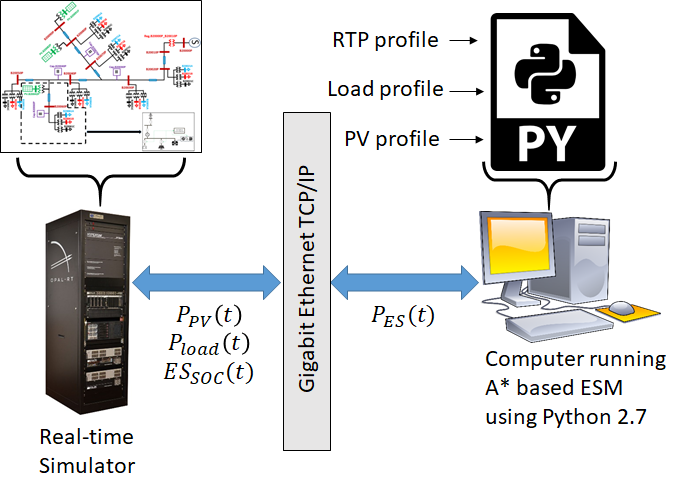
\includegraphics[width = 0.5\linewidth]{figs/A8/RT_block.png}
    \caption{Block layout of the CHIL setup}
    \label{fig:RT_block}
\end{figure}

\begin{figure}[!ht]
    \centering
    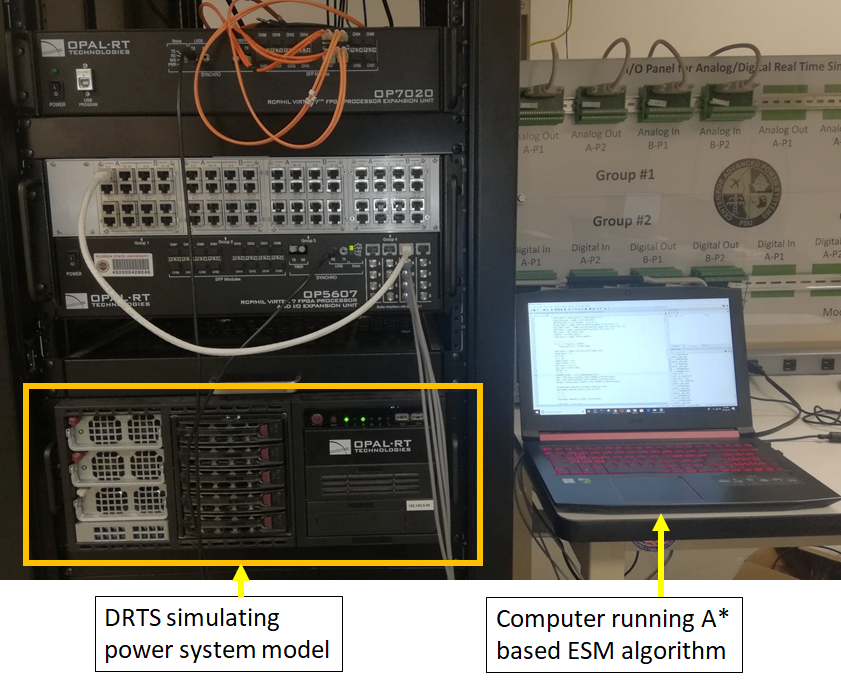
\includegraphics[width = 0.5\linewidth]{figs/A8/LAB_REAL.png}
    \caption{Actual CHIL setup}
    \label{fig:LAB_REAL}
\end{figure}

For the CHIL simulation, the ESM algorithm was set up according to the setup described in Section \ref{OFF}. The simulation was run for 50 hours (200 time steps) in real-time. Fig. \ref{fig:RT_TESTING} shows the real-time and the offline simulation results for the 50-hour run. It can be seen that the real-time simulation result shown by the dotted lines follows the off-line simulation result shown by the solid line. The results are similar to the first two days of Fig. \ref{fig:SBMPO_COMP_10_12} as expected. The comparison of the real-time and offline cost savings of the algorithm is shown in table \ref{tab:rt_cost}. It can be seen from the table that the real-time cost savings are comparable to the offline results.

\begin{figure}[!ht]
    \centering
    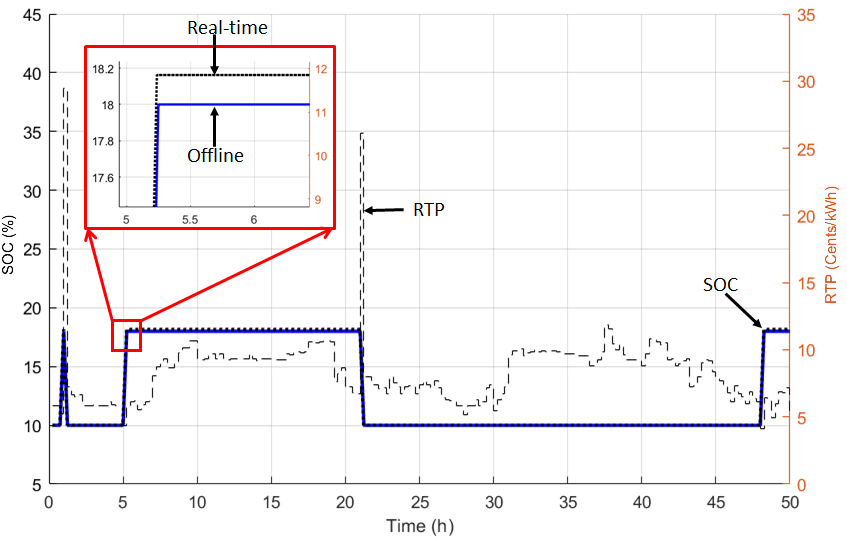
\includegraphics[width = 0.5\linewidth]{figs/A8/RT_TESTING.png}
    \caption{Real-time vs offline result (50  hours)}
    \label{fig:RT_TESTING}
\end{figure}

\begin{table}[htb]
\centering
\caption{Real-time simulation cost (48 hours)}
\label{tab:rt_cost}
\begin{tabular}{l|l|l|l|}
\cline{2-4}
                                          & Real-time & Offline & Difference \\ \hline
\multicolumn{1}{|l|}{Case1}               & \$1,662   & \$1,579 & 4.99\%     \\ \hline
\multicolumn{1}{|l|}{Cas2}                & \$1,713   & \$1,628 & 4.96\%     \\ \hline
\multicolumn{1}{|l|}{A* Case}             & \$1,345   & \$1,286 & 4.39\%     \\ \hline
\multicolumn{1}{|l|}{A* savings (Case 1)} & 19.07\%   & 18.56\% & 0.52\%     \\ \hline
\multicolumn{1}{|l|}{A* savings (Case 2)} & 21.48\%   & 21.01\% & 0.48\%     \\ \hline
\end{tabular}
\end{table}


\chapter{Conclusions and future work}
In this prospectus report, the potential impacts of DER (distributed energy resource) integration on the distribution network has been reviewed. Moreover, the challenges of coordinating the system voltage regulation and optimally managing system energy under a real-time pricing scheme have also been explored. The reviews lead to the identification of gaps in the current methods of voltage regulation and optimum energy management. Consequently, the author proposed two algorithms that would help in the integration of DERs into the grid.

A coordinated voltage control algorithm based on the concepts of electrical distance calculation and voltage sensitivity analysis has been developed and presented. The algorithm proposed, has the ability to coordinate the reactive power reference points for the distributed generation and traditional voltage regulation devices located along the feeder, taking into account their potential impacts on the entire system. By using this approach, a reduction in the use of traditional regulation devices can be achieved and the voltage profiles along the network can be controlled for the most part by just using the already existing DG inverters present on the network. The planned additions to this work are as follows.

\begin{itemize}
    \item Develop a state estimation technique which can determine the system voltage angle from real and reactive power readings.
    \item Perform real-time validation of developed algorithm
\end{itemize}

Moreover, a novel energy management system aimed to determine the optimal operation of a single grid connected DS has been proposed. The management scheme is designed to optimize the charging and discharging of grid-connected energy storage by formulating the problem as a graph search and solving the graph search using the A* search algorithm. The A* based ESM is tested using real data collected from the SUNGRIN project, NYISO, and PG\&E. It also considers both a net metering scenario and a different sell back price scenario where the buying price of energy is different from the selling price.  The planned additions to this work are as follows.

\begin{itemize}
    \item develop an algorithm capable of dealing with multiple sources while maintaining system constraints.
    \item Perform real-time validation with multiple sources.
\end{itemize}

% \section{Current state of the work}
% In the current state the author has developed ...
%\section{Future Work Schedule}


\section{Publications}
\subsection{Accepted conference paper}
\begin{itemize}
    \item A. Newaz, J. Ospina and M. O. Faruque. Coordinated Voltage Control in Distribution
Systems with Distributed Generations. [Accepted] \textit{IEEE PES General Meeting,2019}.
\end{itemize}


\subsection{Submitted Journal Paper}
\begin{itemize}
    \item A. Newaz, J. Ospina and M. O. Faruaue. A Graph Search Based Optimal Control Technique for Enterprise Level Energy Storage Based on Forecasting of PV, Load and Real-Time price of Energy. [Submitted] \textit{IEEE transaction on industrial electronics.}

\end{itemize}

%\subsection{Paper under construction}
\subsection{Future Work and Schedule}
In the upcoming time, real-time validation of the coordinated voltage control algorithm will be performed and the results will be published. The graph search based energy management system will be updated to include multiple DERs and system constraints. A grantt chart for important milestones is shown in fig. \ref{fig:GANTT}.

\begin{figure}[!ht]
    \centering
    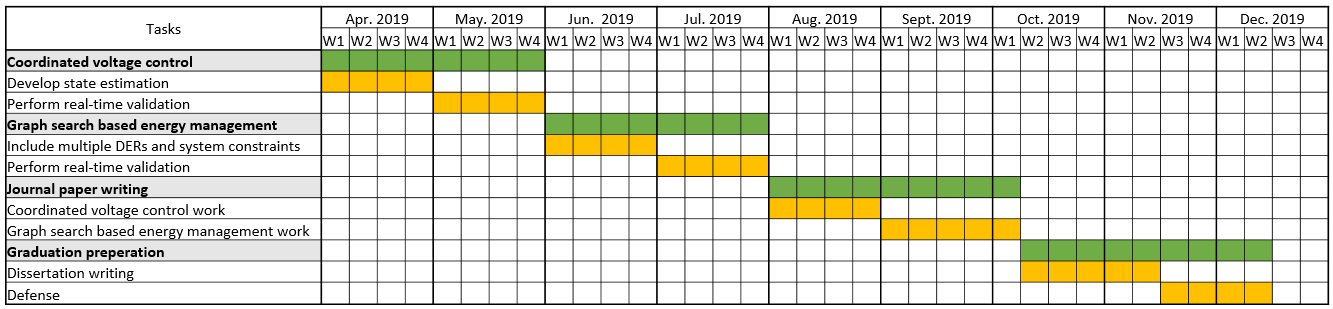
\includegraphics[width = 1.3\linewidth, angle =270]{figs/GANTT.png}
    \caption{Grantt chart for future tasks}
    \label{fig:GANTT}
\end{figure}


% \chapter{Development of Graph Search Based Energy Management for Multiple Interconnected DERs}
% \section{Problem formulation}
% \section{Control architecture}
% \subsection{DC power flow}
% \subsection{Hybrid Optimization using DC power-flow and A*}

% \section{Offline Validation}
% \section{Real-time Validation}




% \chapter{Conclusion and Future Work}



%\input chapter1
%\input chapter2
%\input chapter3

%\appendix
%\input appendix1

% You have your choice of bibliography sections, either
% hand-crafted or BibTeX.

% Or use the BibTeX bibliography/references section below.  View the
% file 'myrefs.bib' to get a feel for what these entries may look
% like.  See the document in the 'sample' folder for more citation and
% BibTeX examples.

\bibliographystyle{unsrt}
\bibliography{INTRO,A8,CVC,LR,TRUE_BIB}

\begin{biosketch}
%This is my biography.
\end{biosketch}

\end{document}
